\chapter{Experimental Results}\label{exp_results_chapter}

\section{Setup}

Prior to discussing about the actual performance and peculiarities of each estimator, it is important to give at least a brief introduction about the experimental setup, library and data-wise, used to achieve such results.

\subsection{Coding Environment and Libraries}

Jupyter Notebook, integrated in Jetbrain's DataSpell IDE, was used for the development of every major phase of the assignment, supported by some basic Python source files containing utility functions and the required implementations of the KNN and NaiveBayes classifiers.
Additionally, the project mainly makes use of the following Python libraries:

\begin{itemize}
    \item \textit{numpy}, \textit{pandas} to efficiently manipulate data

    \item \textit{sklearn} for training and evaluation metrics utilities, as well as the implementations of the Support Vector Machine Classifier and Random Forest Classifier

    \item \textit{seaborn} and \textit{plotly} plotting libraries to create useful charts, as well as \textit{kaleido} to allow to export plotly charts to images.
\end{itemize}


\subsection{MNIST Digits Dataset}

The dataset that this assignment is centered on is the MNIST handwritten digits dataset, consisting of 70k images pre-divided into two tranches of 60k and 10k, respectively for training and testing of machine learning models. Each image is represented by a 784-dimensional vector, which corresponds to a $28 \times 28$ pixels image. Such an image, additionally is grayscale and single channel, as opposed to the common triple channel (rgb) representation for colored images.

\begin{figure}[h]
    \centering
    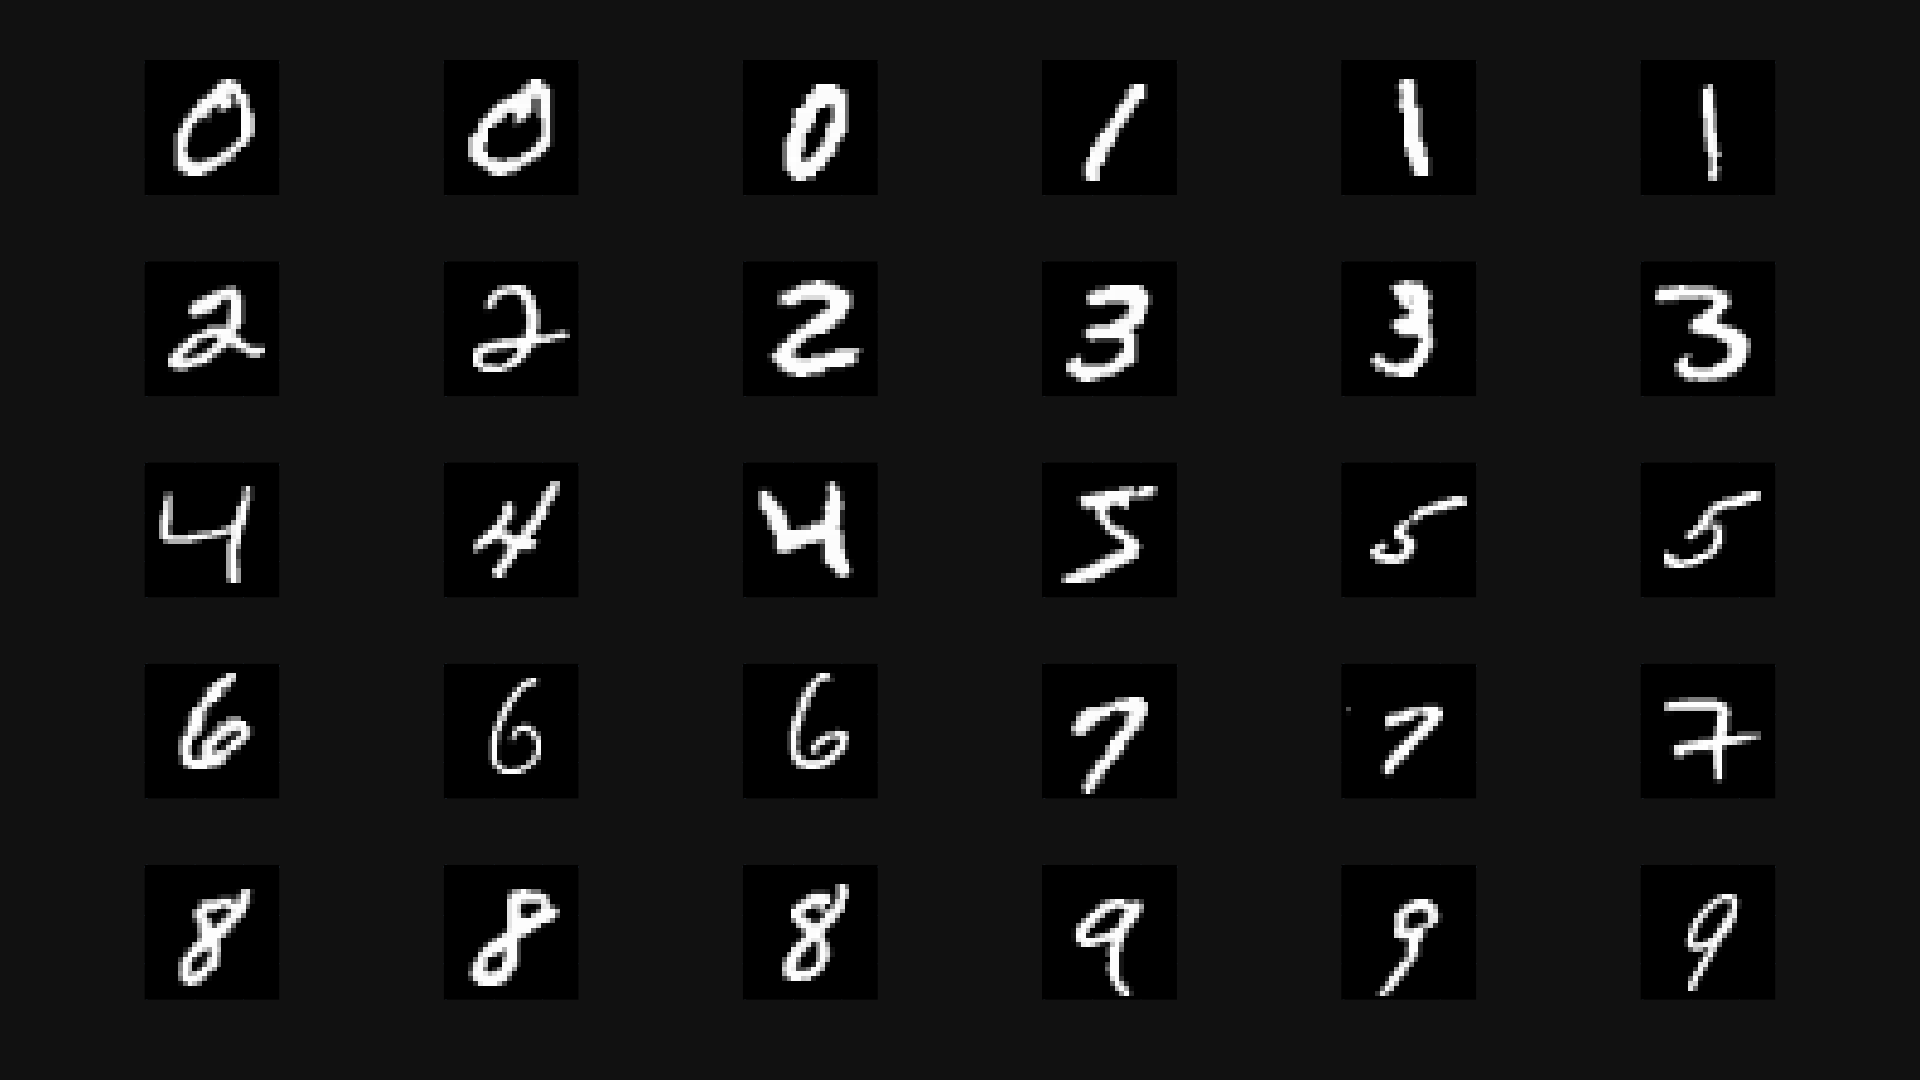
\includegraphics[scale=0.15]{images/mnist-data/digit-samples.png}
    \caption{Some sample images from the MNIST handwritten digits dataset}
    \label{fig:mnist_data_image_samples}
\end{figure}

\subsubsection{Train and Test Split}

As aforementioned, the dataset was already divided in 60k images for traning and 10k for testing. Such partitions were the most commonly used during the main phases of the project, however, some exceptions were made during the validation and hyperparameters tuning phase of some models: since the training or inference time and memory requirements of some classifiers scaled superlinearly with respect to the dimension of the input dataset, it was deemed appropriate to use a smaller version of the dataset, corresponding to a stratified sample of the of 6000 images, taken from the full training set. In particular, this shrunk dataset was used with the following classifiers:

\begin{itemize}
    \item SVM, because of its approximately quadratic space complexity and cubic time complexity of the training phase
    
    \item KNN, because of its approximately quadratic time complexity of the prediction, hence testing, phase
\end{itemize}

It is noted, however, that, after the best parameters were identified, every model was trained with the full training set and tested against the full testing set.

\subsubsection{Data Engineering}

The dataset was analyzed in terms of feature distributions and missing or dirty values, but it was found to be particularly clean and well balanced: this is to be expected because of its vast popularity and its educational purpose.
Each feature was originally in the interval $[0, 255]$, only to be successively scaled down using a min-max approach into the $[0, 1]$ interval. This is a relevant detail, because almost all the classifiers relied on some definition of distance, and are to generally perform better if the data is properly scaled.
Another engineering intervention was performed to remove features that were constantly 0 in value: by taking a look at some sample images, it could be seen that there were spaces that were consistently black (0), usually representing padding. A feature that is constant in value doesn't have predictive power, so such pixels, 65 in total, were removed, leaving the dataset with 719 out of the 784 original features.

\subsection{Halving Gridsearch for Hyperparameter Tuning}

The tuning of hyperparameters was achieved by using \textit{sci-kit learn}'s \textit{HalvingGridSearchCV} class, which is an experimental variant of \textit{GridSearchCV}. The main peculiarity of this approach is the \textit{halving} part, indicating that, in a parameterized number of iterations, the amount of estimators used in the optimal parameters search is halved (only the best ones go forward), while the number of resources allocated for the training and validation phases is doubled. This leads to faster execution times when compared to the basic Grid Search with Cross Validation procedure, while the quality of the results is about equal.
Below is an image from the sklearn documentation that allows to visualize how the halving grid search works.

\begin{figure}[h]
    \centering
    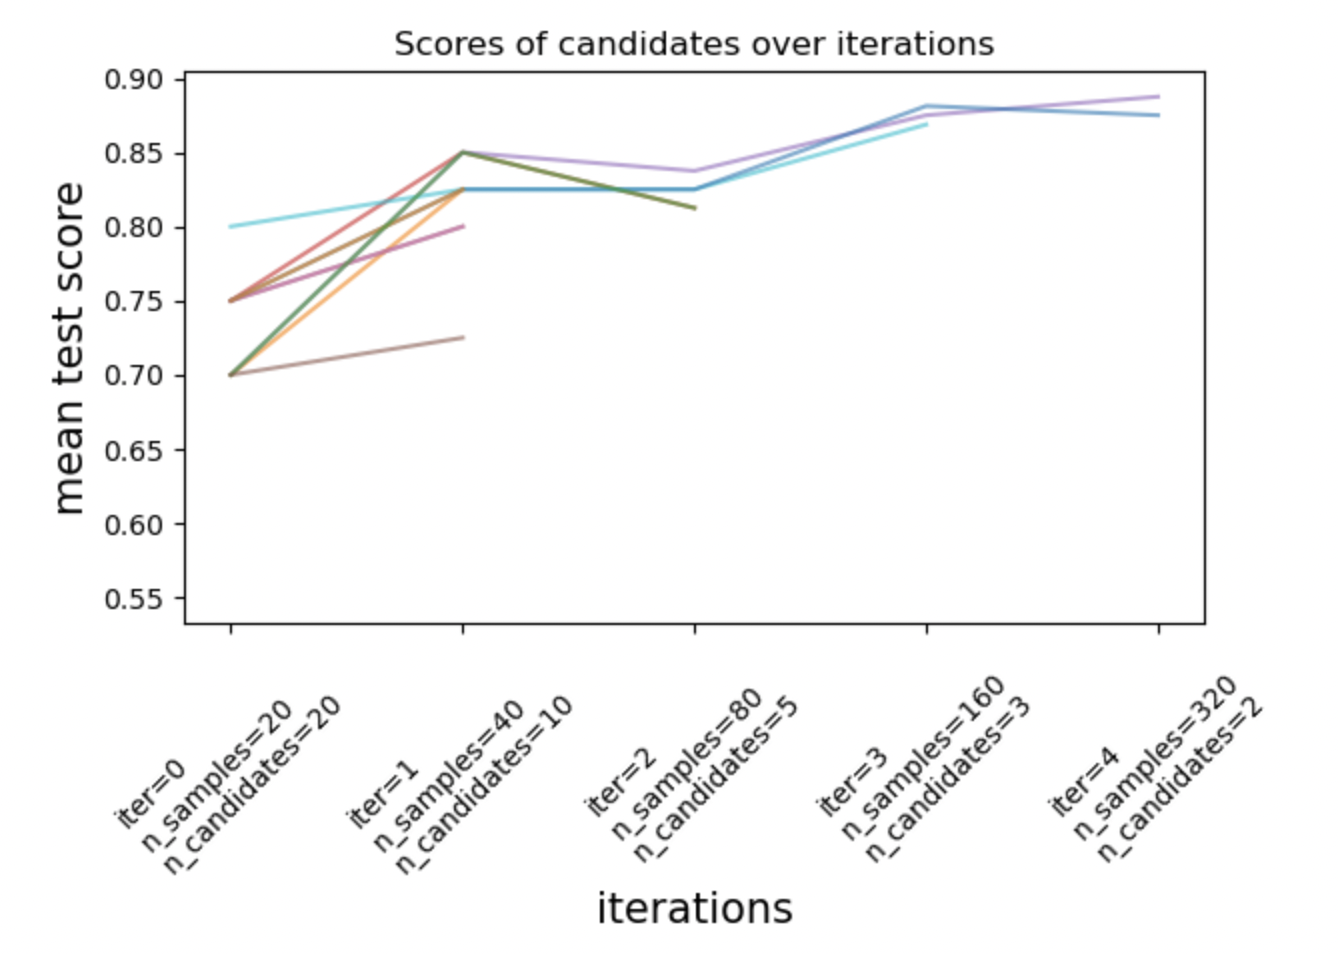
\includegraphics[scale=0.4]{images/halving-grid-search/sklearn-halving-grid-search-visual.png}
    \caption{Visual representation of the Halving Grid Search with CV Procedure}
    \label{fig:halving_grid_search_cv}
\end{figure}

\subsection{Evaluation Metrics}

Two evaluation metrics were mainly used to test the models:

\begin{itemize}
    \item \textit{Accuracy}, chosen because false negatives are acceptable and the dataset is well balanced: each of the 10 classes occurs in about 10\% of the samples, meaning that they are almost equally distributed. \textit{F1-Score} was also considered in some tests, but it was just to check for any anomalous behavior that accuracy isn't able to highlight; indeed, nothing to note was found.
    
    \item \textit{Confusion Matrix}, chosen to better grasp which classes were the most easy or difficult to predict by each classifier.
\end{itemize}


\break
\section{Random Forest}

\subsection{Implementation}

As mentioned previously, \textit{sci-kit learn}'s \textit{RandomForestClassifier} implementation was the one used for this assignment. It was chosen because assignment's instruction allowed it, and it offered a convenient API as well as easy support for parallelization.

\subsection{Hyperparameter Tuning}

The following hyperparameters set was chosen to perform the grid search on:

\begin{figure}[h]
    \centering
    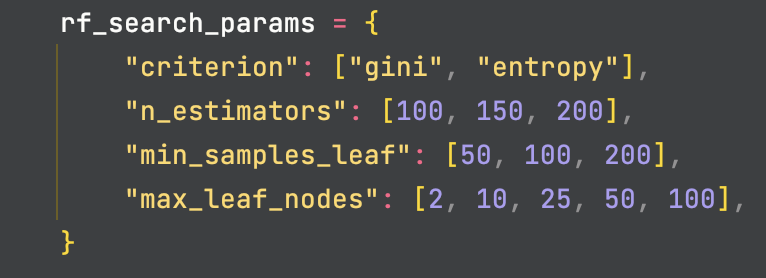
\includegraphics[scale=0.7]{images/exp-results/rf/rf-params.png}
    \caption{RandomForestClassifier grid search parameters}
    \label{fig:exp_res_rf_params}
\end{figure}

The overall set of hyperparameters was somewhat restricted because of constraints on the available computational resources, hence it was focused down to what was empirically found to be the most effective parameter types and values.

More documentation on the meaning of each hyperparameter can be found at the following link: \url{https://scikit-learn.org/stable/modules/generated/sklearn.ensemble.RandomForestClassifier.html#sklearn.ensemble.RandomForestClassifier}

\paragraph{Best Parameters} The grid search found the \textit{RandomForestClassifier} with the following parameters to be the best one:

\begin{lstlisting}[language=json]
{
    "criterion": "gini",
    "n_estimators": 200,
    "min_samples_leaf": 50,
    "max_leaf_nodes": 100
}
\end{lstlisting}

\subsection{Performance Metrics}

\paragraph{Overall Accuracy} The overall accuracy of the model was $91.87\%$

\paragraph{Confusion Matrix} Below is the confusion matrix for the \textit{RandomForestClassifier}. It can be noted that it performed very well at labelling 0s and 1s, and relatively poorly at labelling 5s.

\begin{figure}[h]
    \centering
    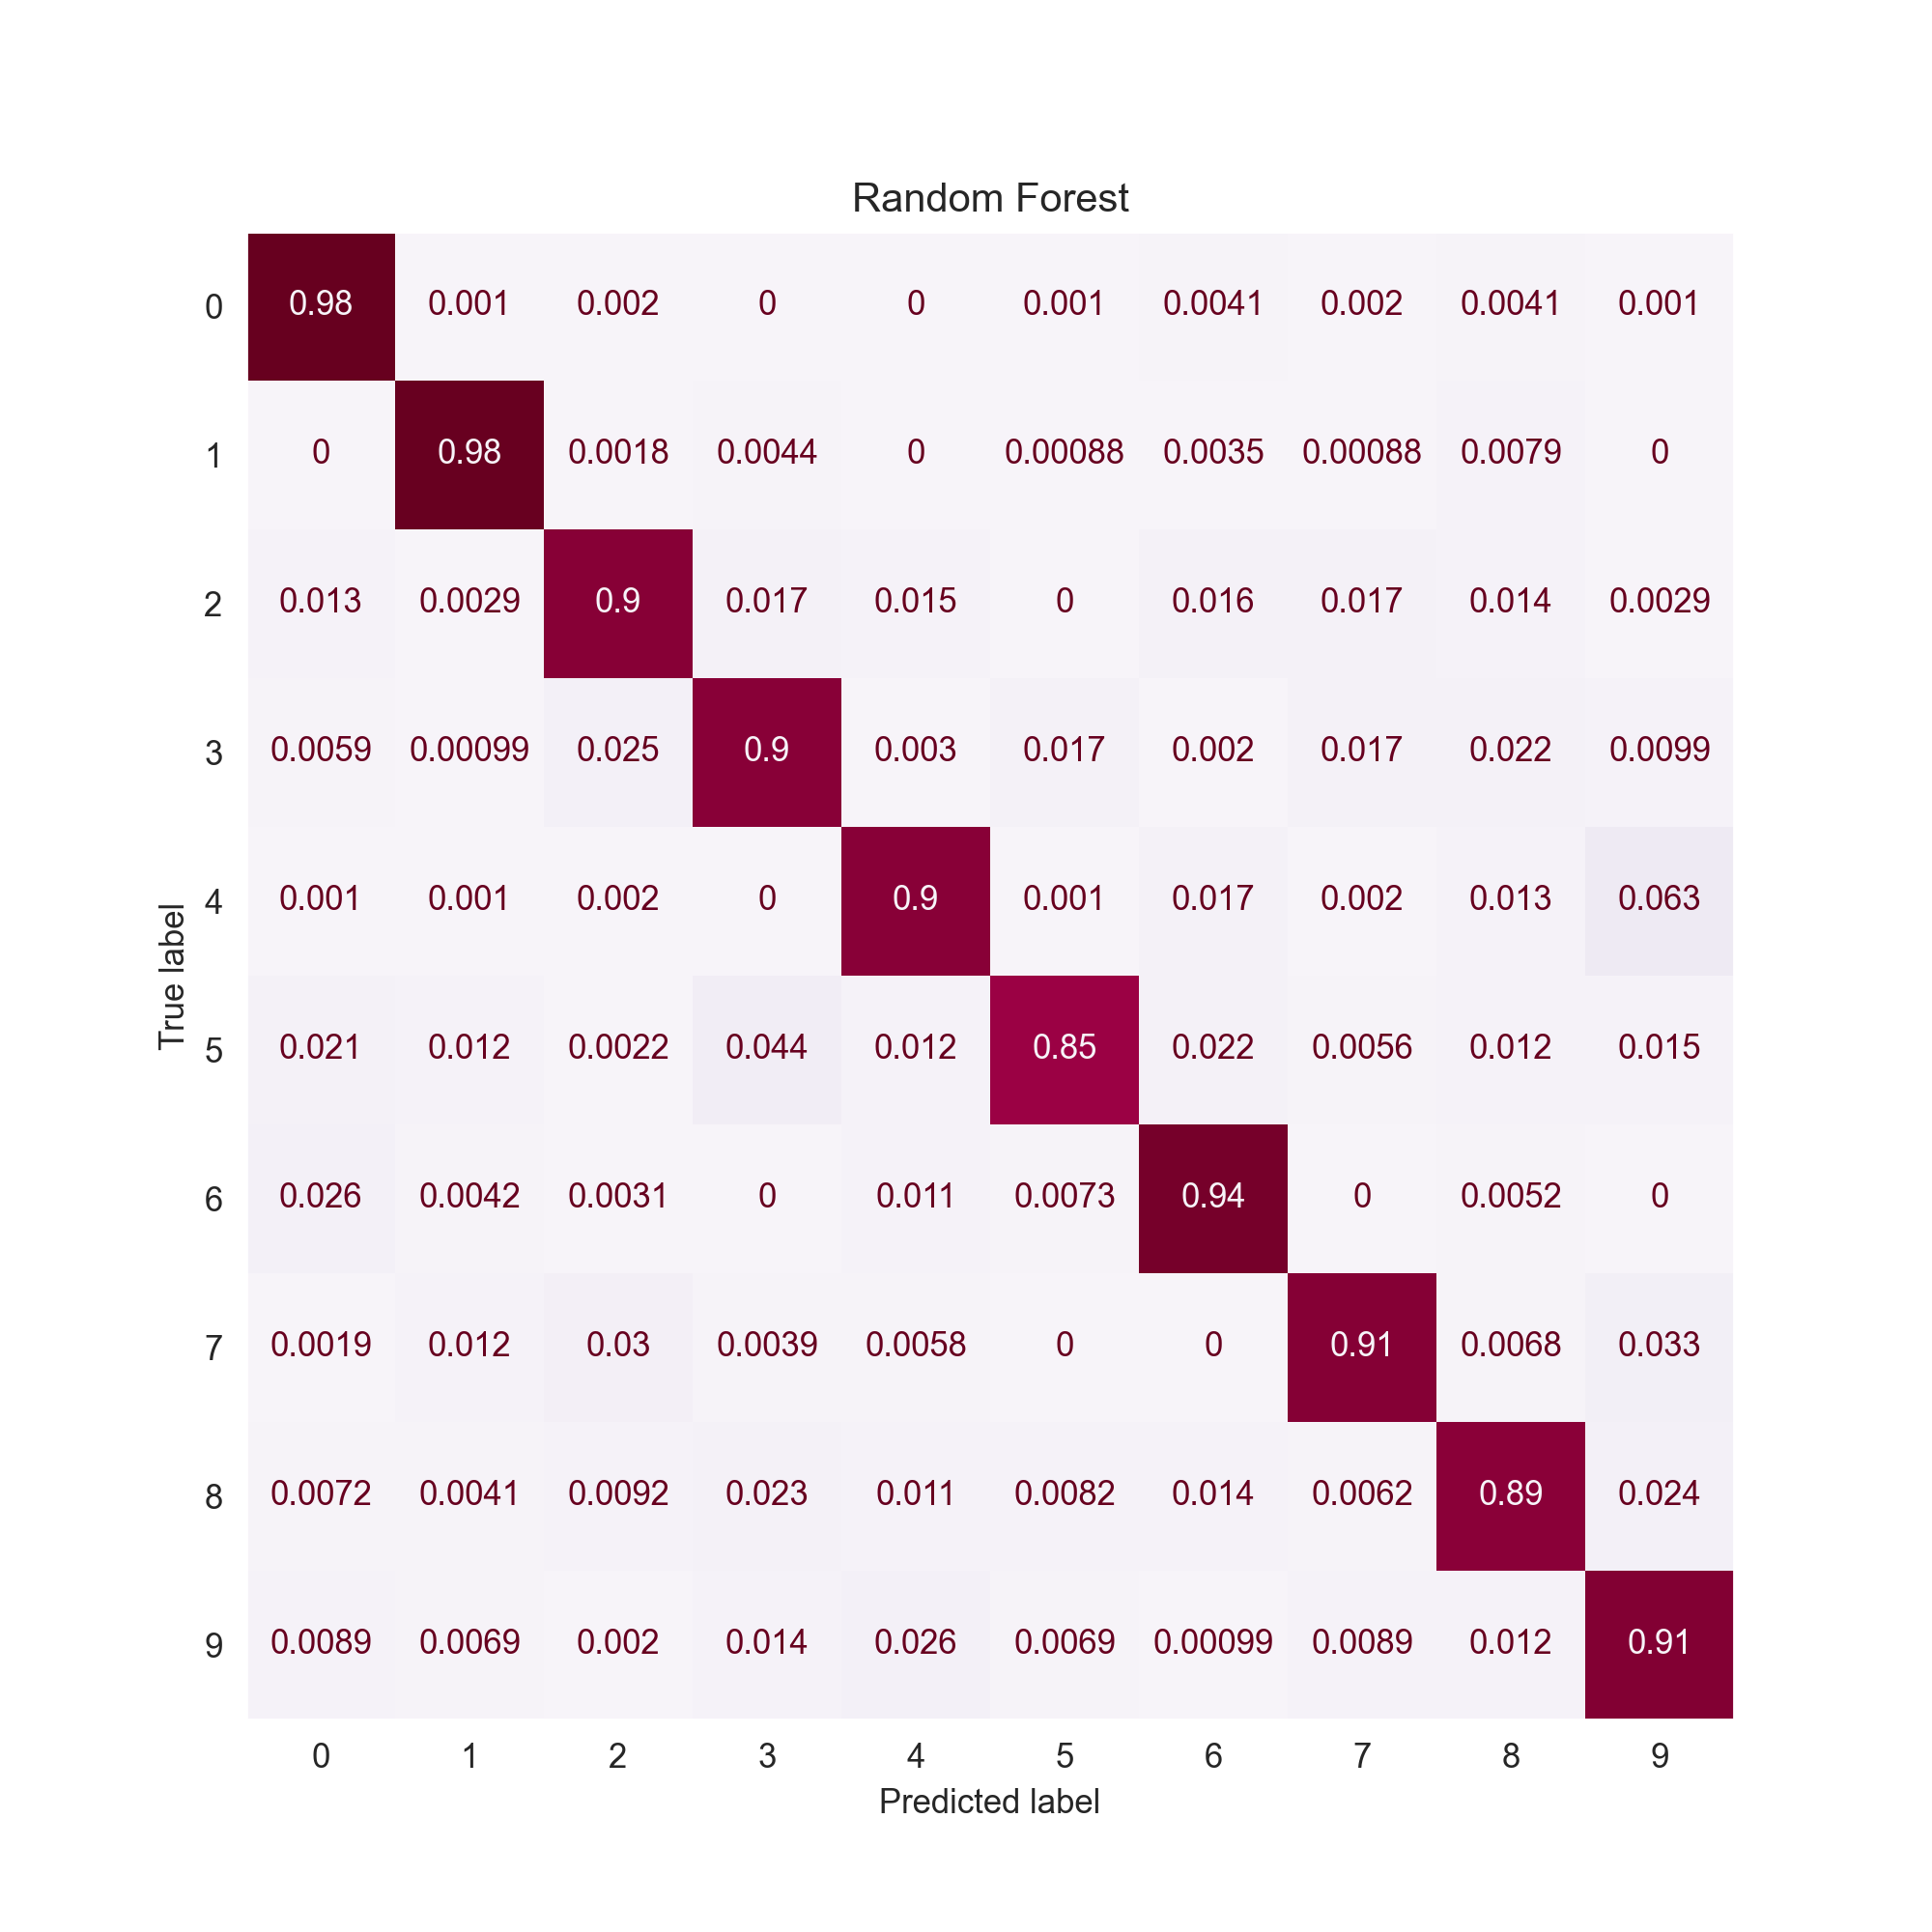
\includegraphics[scale=0.65]{images/exp-results/rf/rf_conf-matrix.png}
    \caption{RandomForestClassifier confusion matrix}
    \label{fig:exp_res_rf_conf_mat}
\end{figure}


\newpage
\section{SVM}

As mentioned previously, \textit{sci-kit learn}'s \textit{SVC} implementation was the one used for this assignment. It was chosen because assignment's instruction allowed it, and it offered a convenient API.

\subsection{Hyperparameter Tuning}

For each type of kernel, the following hyperparameters set was chosen to perform the grid search on:

\begin{lstlisting}[language=json]
{
    "C": [0.05, 0.2, 0.5, 1, 2.5]
}
\end{lstlisting}

The overall set of hyperparameters was limited to just the $C$ parameter, which defines the hardness of the margin, because of the expensiveness of the validation procedure.
Even though results could have been further optimized, a good tradeoff between training time and performance was eventually reached.

\paragraph{Best Parameters} The grid search found that the values of $C$ that were best for each type of \textit{SVM} kernel were the following:

\begin{itemize}
    \item \textbf{Linear Kernel} $\rightarrow C = 0.05$ 

    \item \textbf{Polynomial (2nd Degree) Kernel} $\rightarrow C = 2.5$ 

    \item \textbf{RBF Kernel} $\rightarrow C = 2.5$ 
\end{itemize}

\subsection{Performance Metrics}

The discussion of the performance of the SVM models is divided by the type of kernel that was used to build the model.

\subsubsection{Linear Kernel}

\paragraph{Overall Accuracy} The overall accuracy of the model was $94.66\%$

\paragraph{Confusion Matrix} Below is the confusion matrix for the \textit{Linear Kernel SVM}. It can be noted that it performed very well at labelling 0s and 1s, and relatively poorly at labelling 5s and 8s.

\begin{figure}[h]
    \centering
    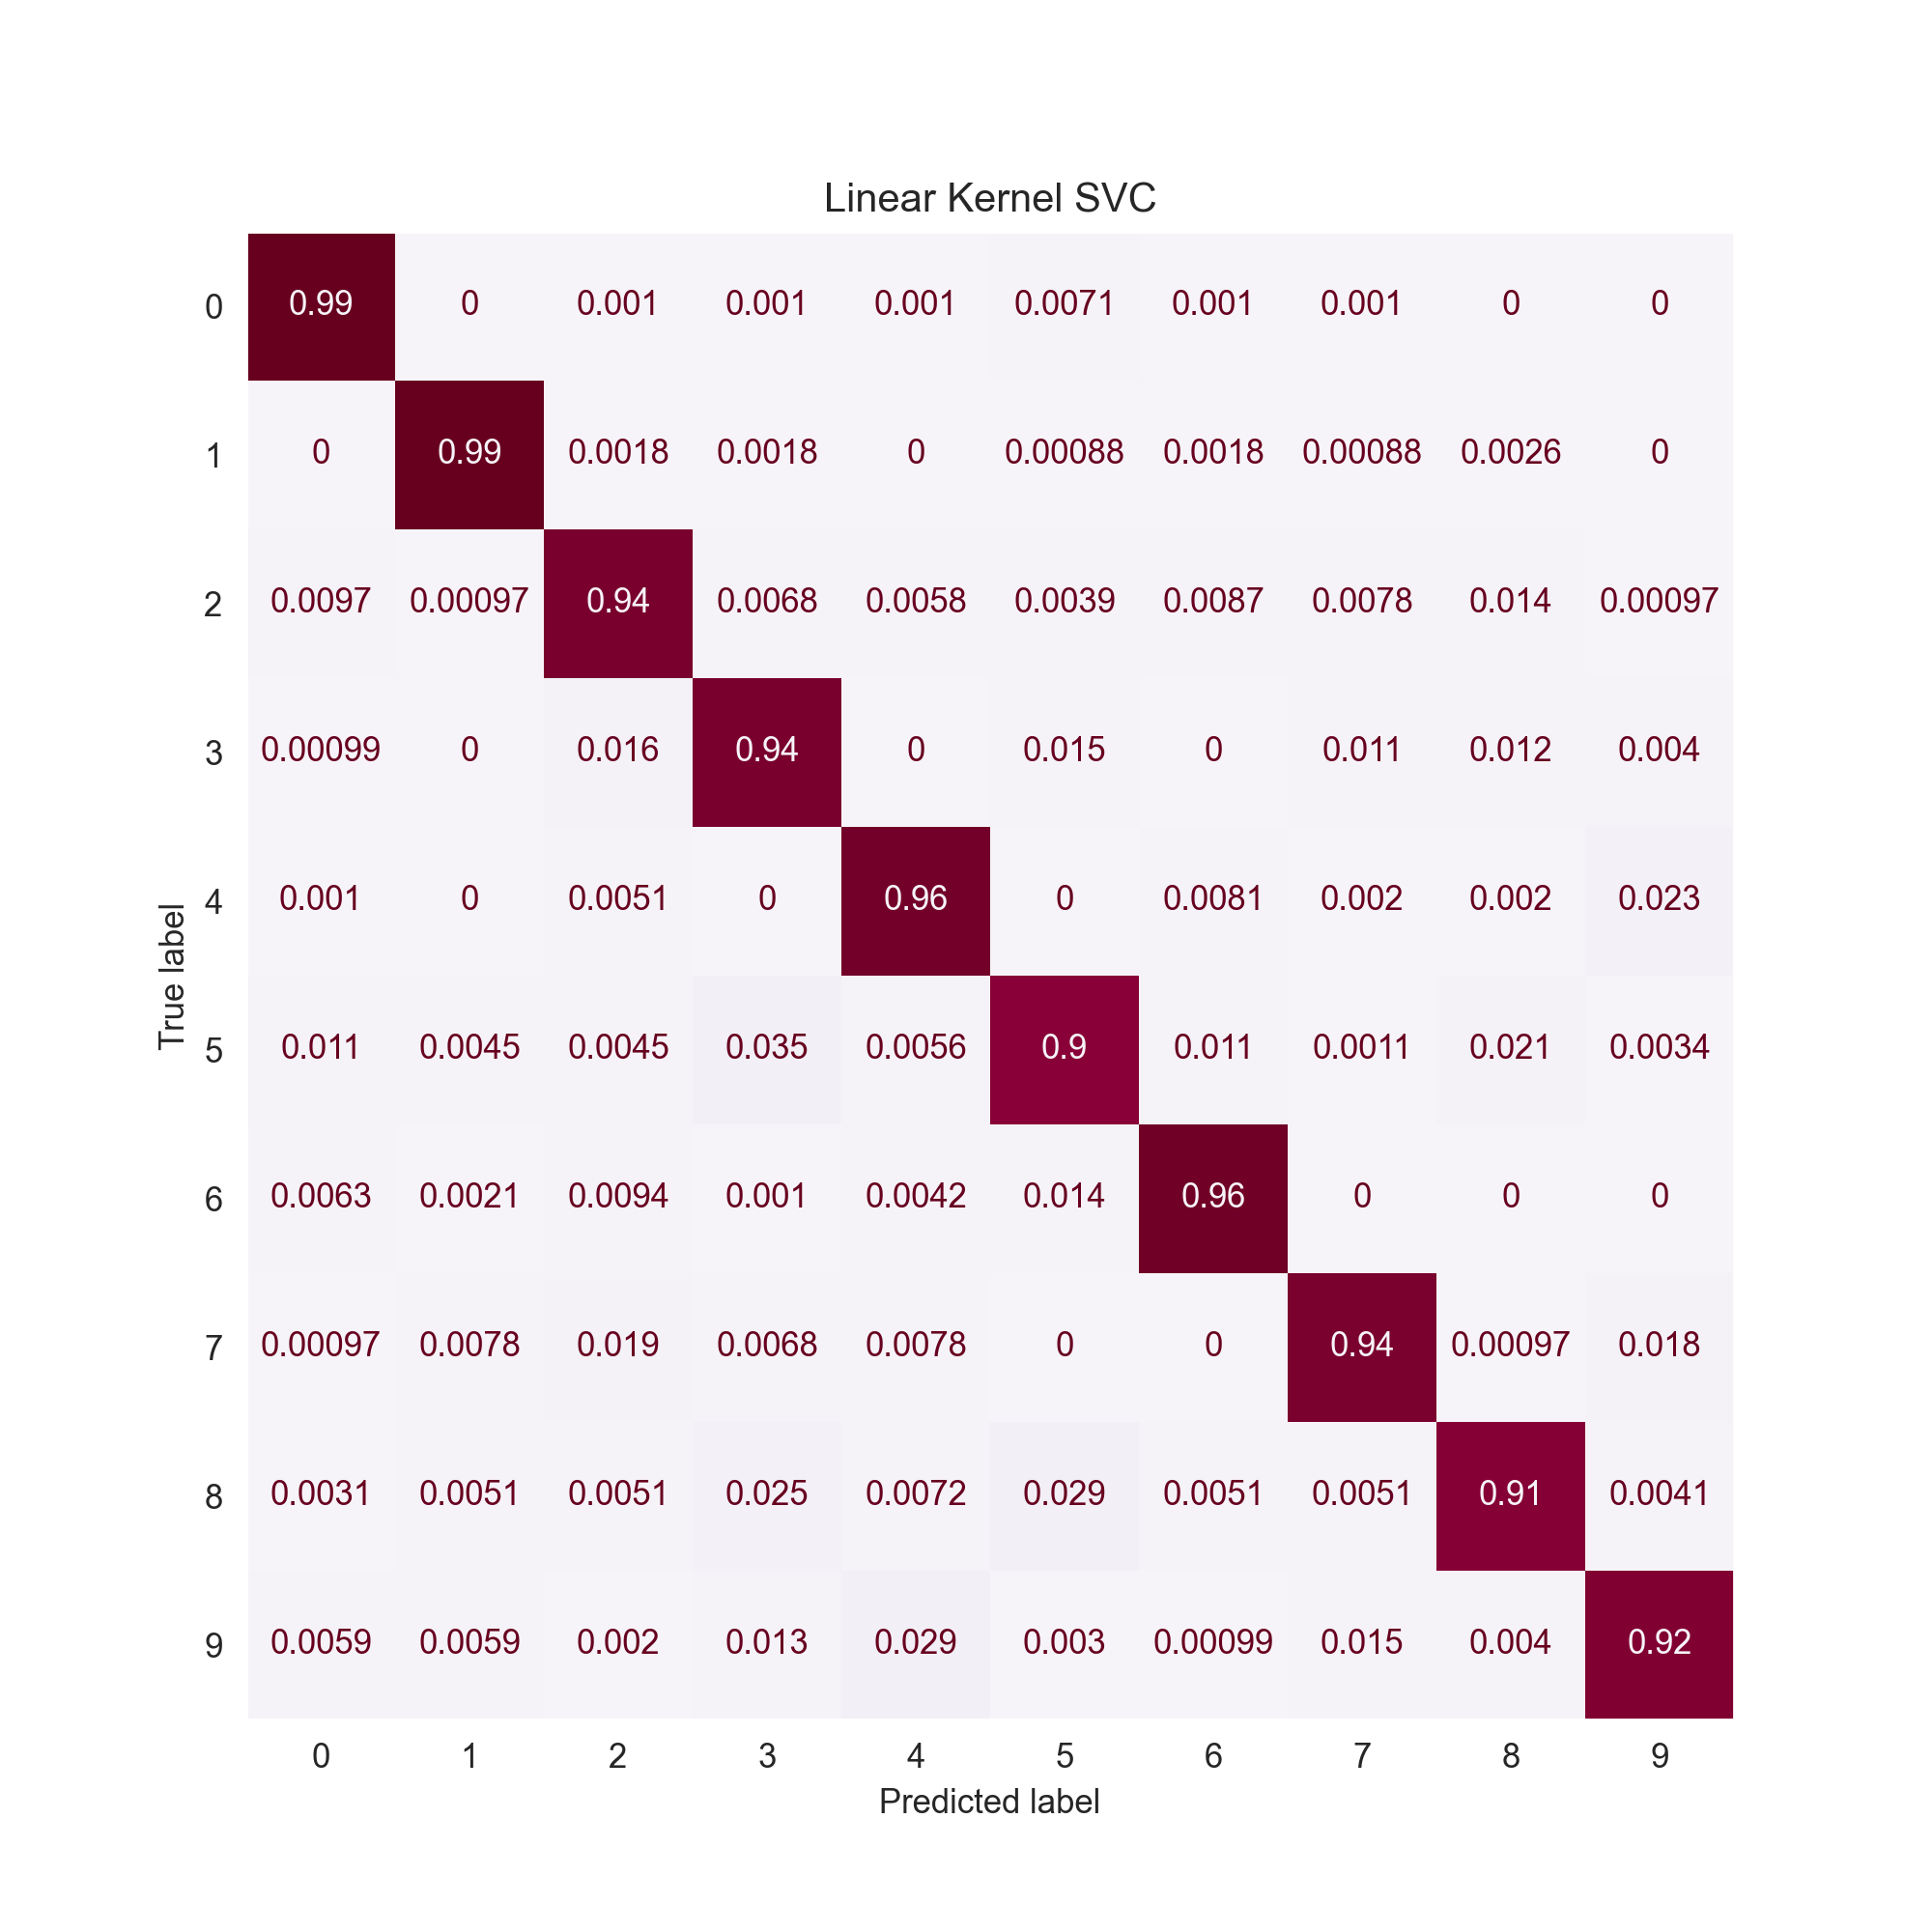
\includegraphics[scale=0.65]{images/exp-results/svm/svc_linear_conf-matrix.png}
    \caption{Linear Kernel SVM confusion matrix}
    \label{fig:exp_res_lin_svm_conf_mat}
\end{figure}

\subsubsection{Polynomial (2nd Degree) Kernel}

\paragraph{Overall Accuracy} The overall accuracy of the model was $94.01\%$

\paragraph{Confusion Matrix} Below is the confusion matrix for the \textit{Polynomial Kernel SVM}. It can be noted that it performed very well at labelling 0s and 1s, and relatively poorly at labelling 2s, 7s, 8s, 9s.

\begin{figure}[h]
    \centering
    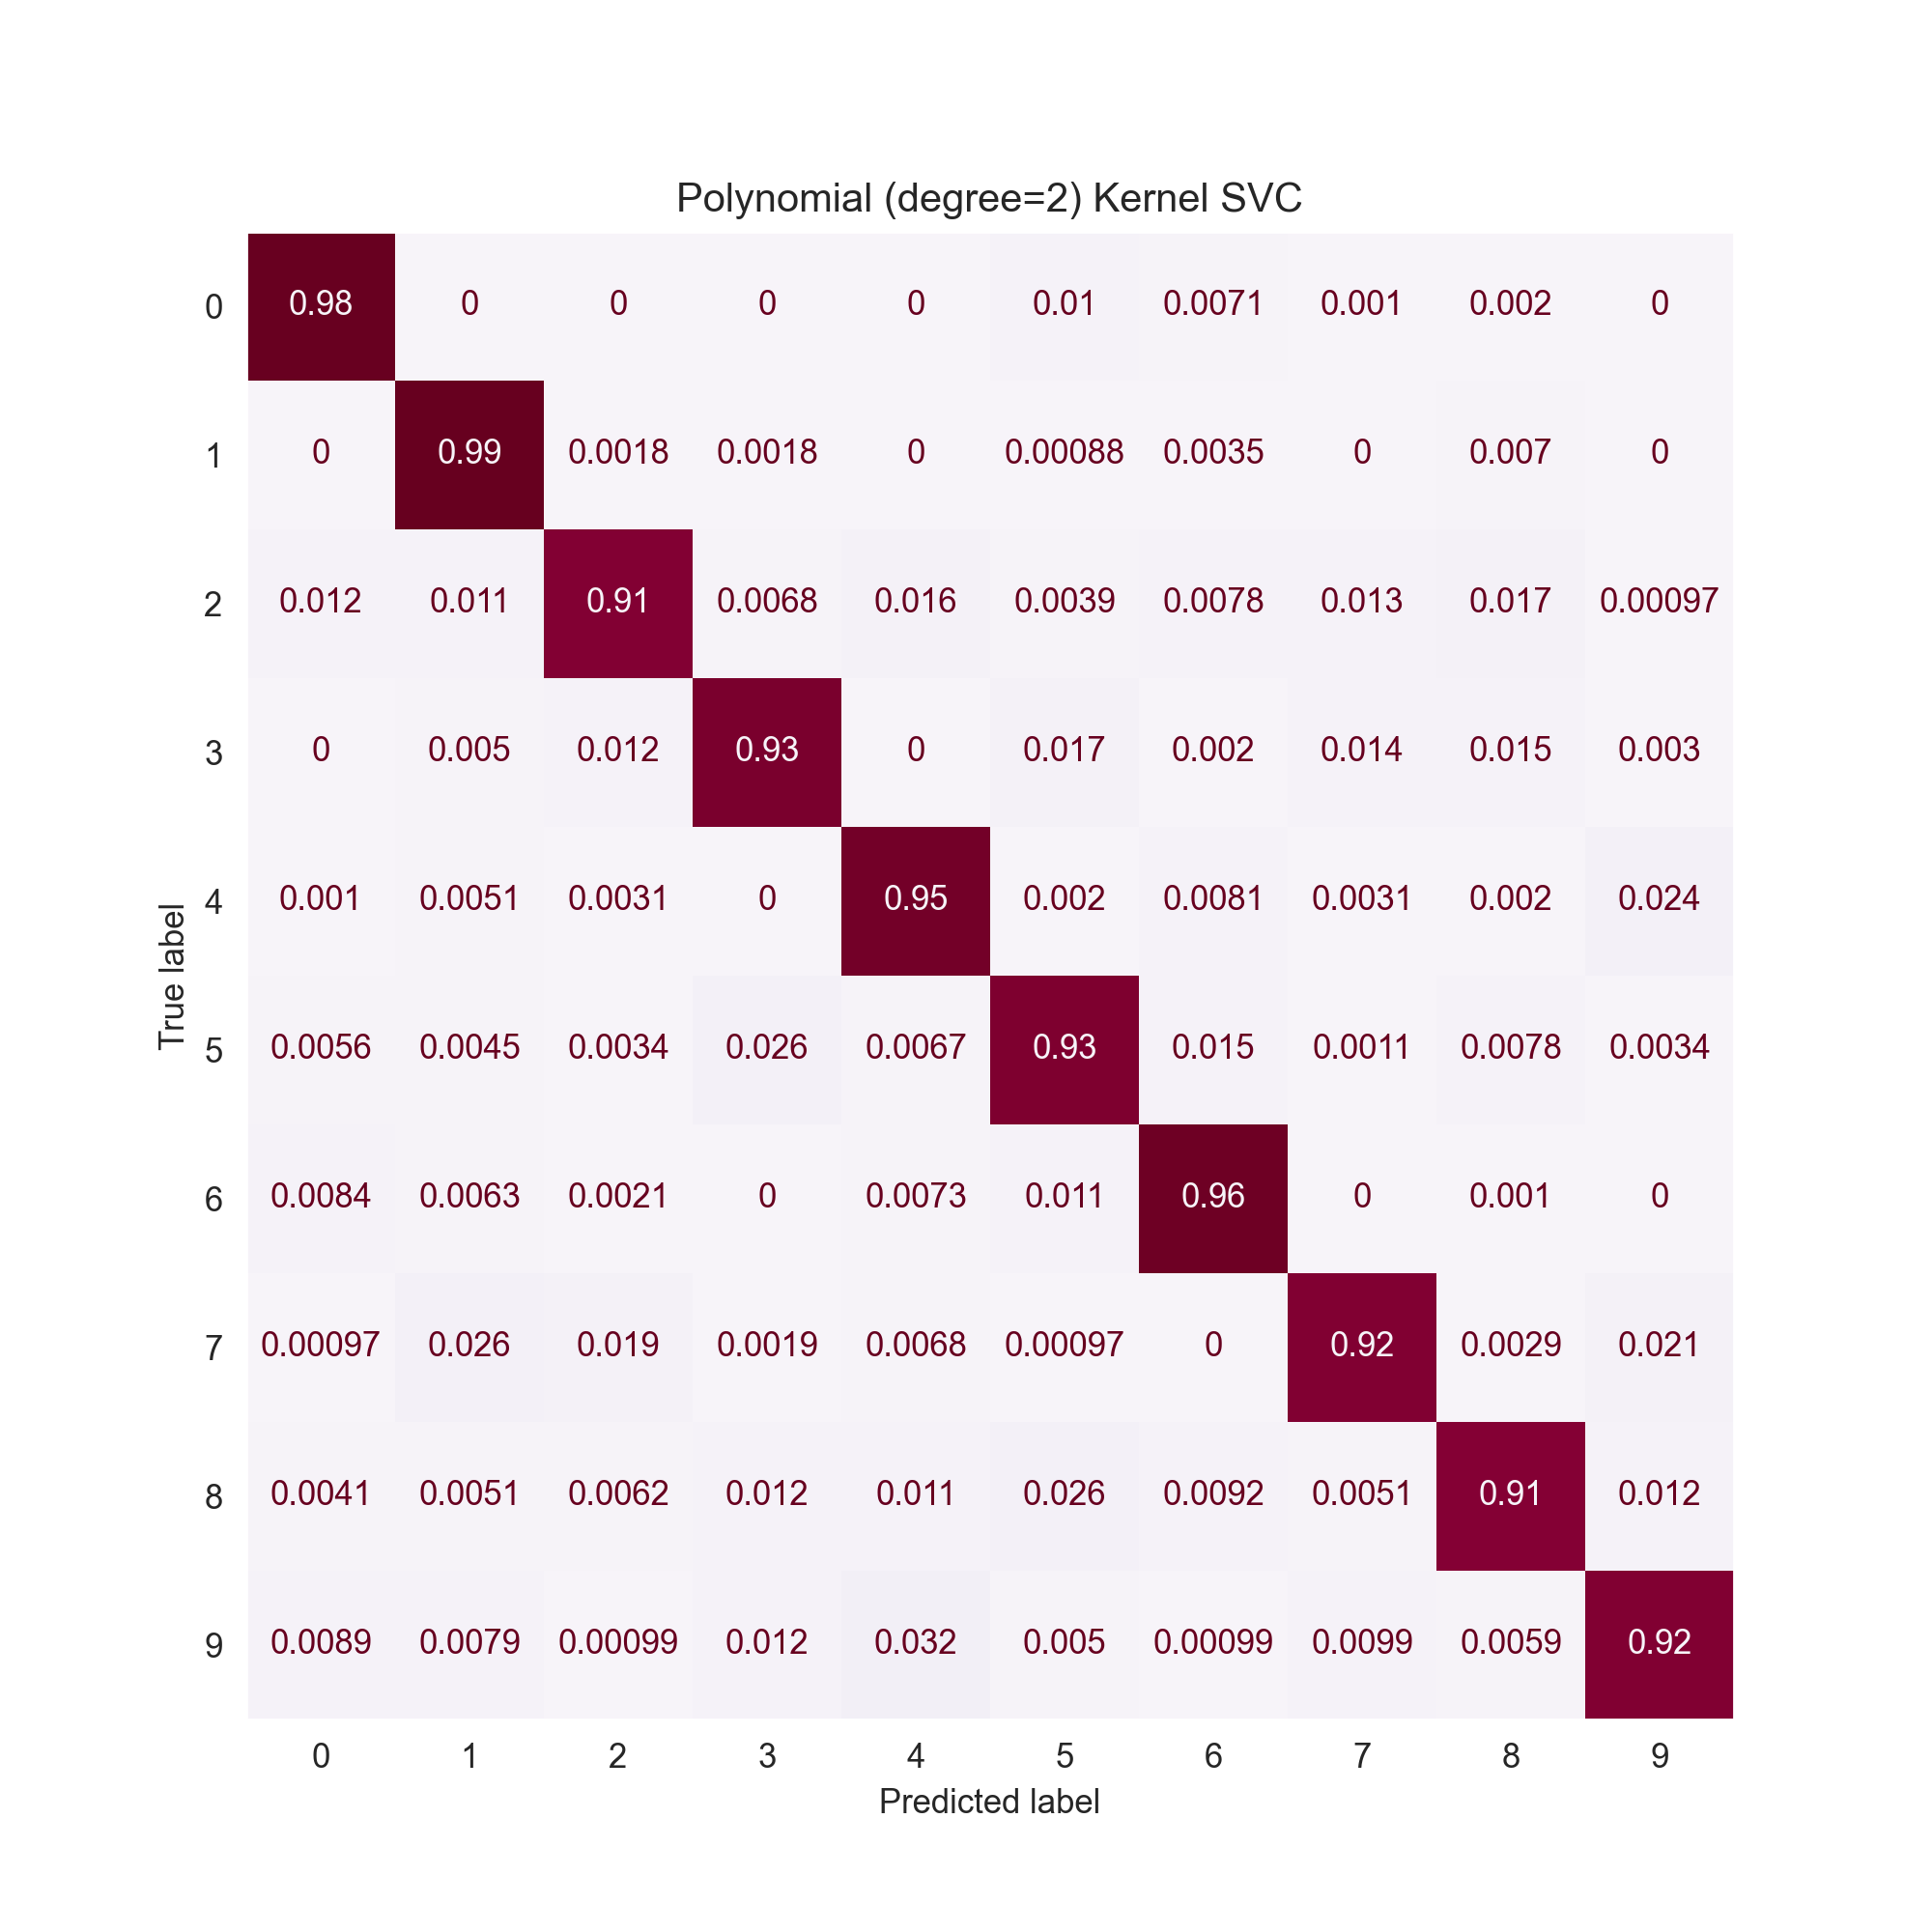
\includegraphics[scale=0.65]{images/exp-results/svm/svc_poly_conf-matrix.png}
    \caption{Polynomial (2nd Degree) Kernel SVM confusion matrix}
    \label{fig:exp_res_poly_svm_conf_mat}
\end{figure}

\subsubsection{Radial Basis Function Kernel}

\paragraph{Overall Accuracy} The overall accuracy of the model was $95.22\%$

\paragraph{Confusion Matrix} Below is the confusion matrix for the \textit{RBF Kernel SVM}. It can be noted that it performed very well at labelling 0s and 1s, and relatively poorly at labelling 5s.

\begin{figure}[h]
    \centering
    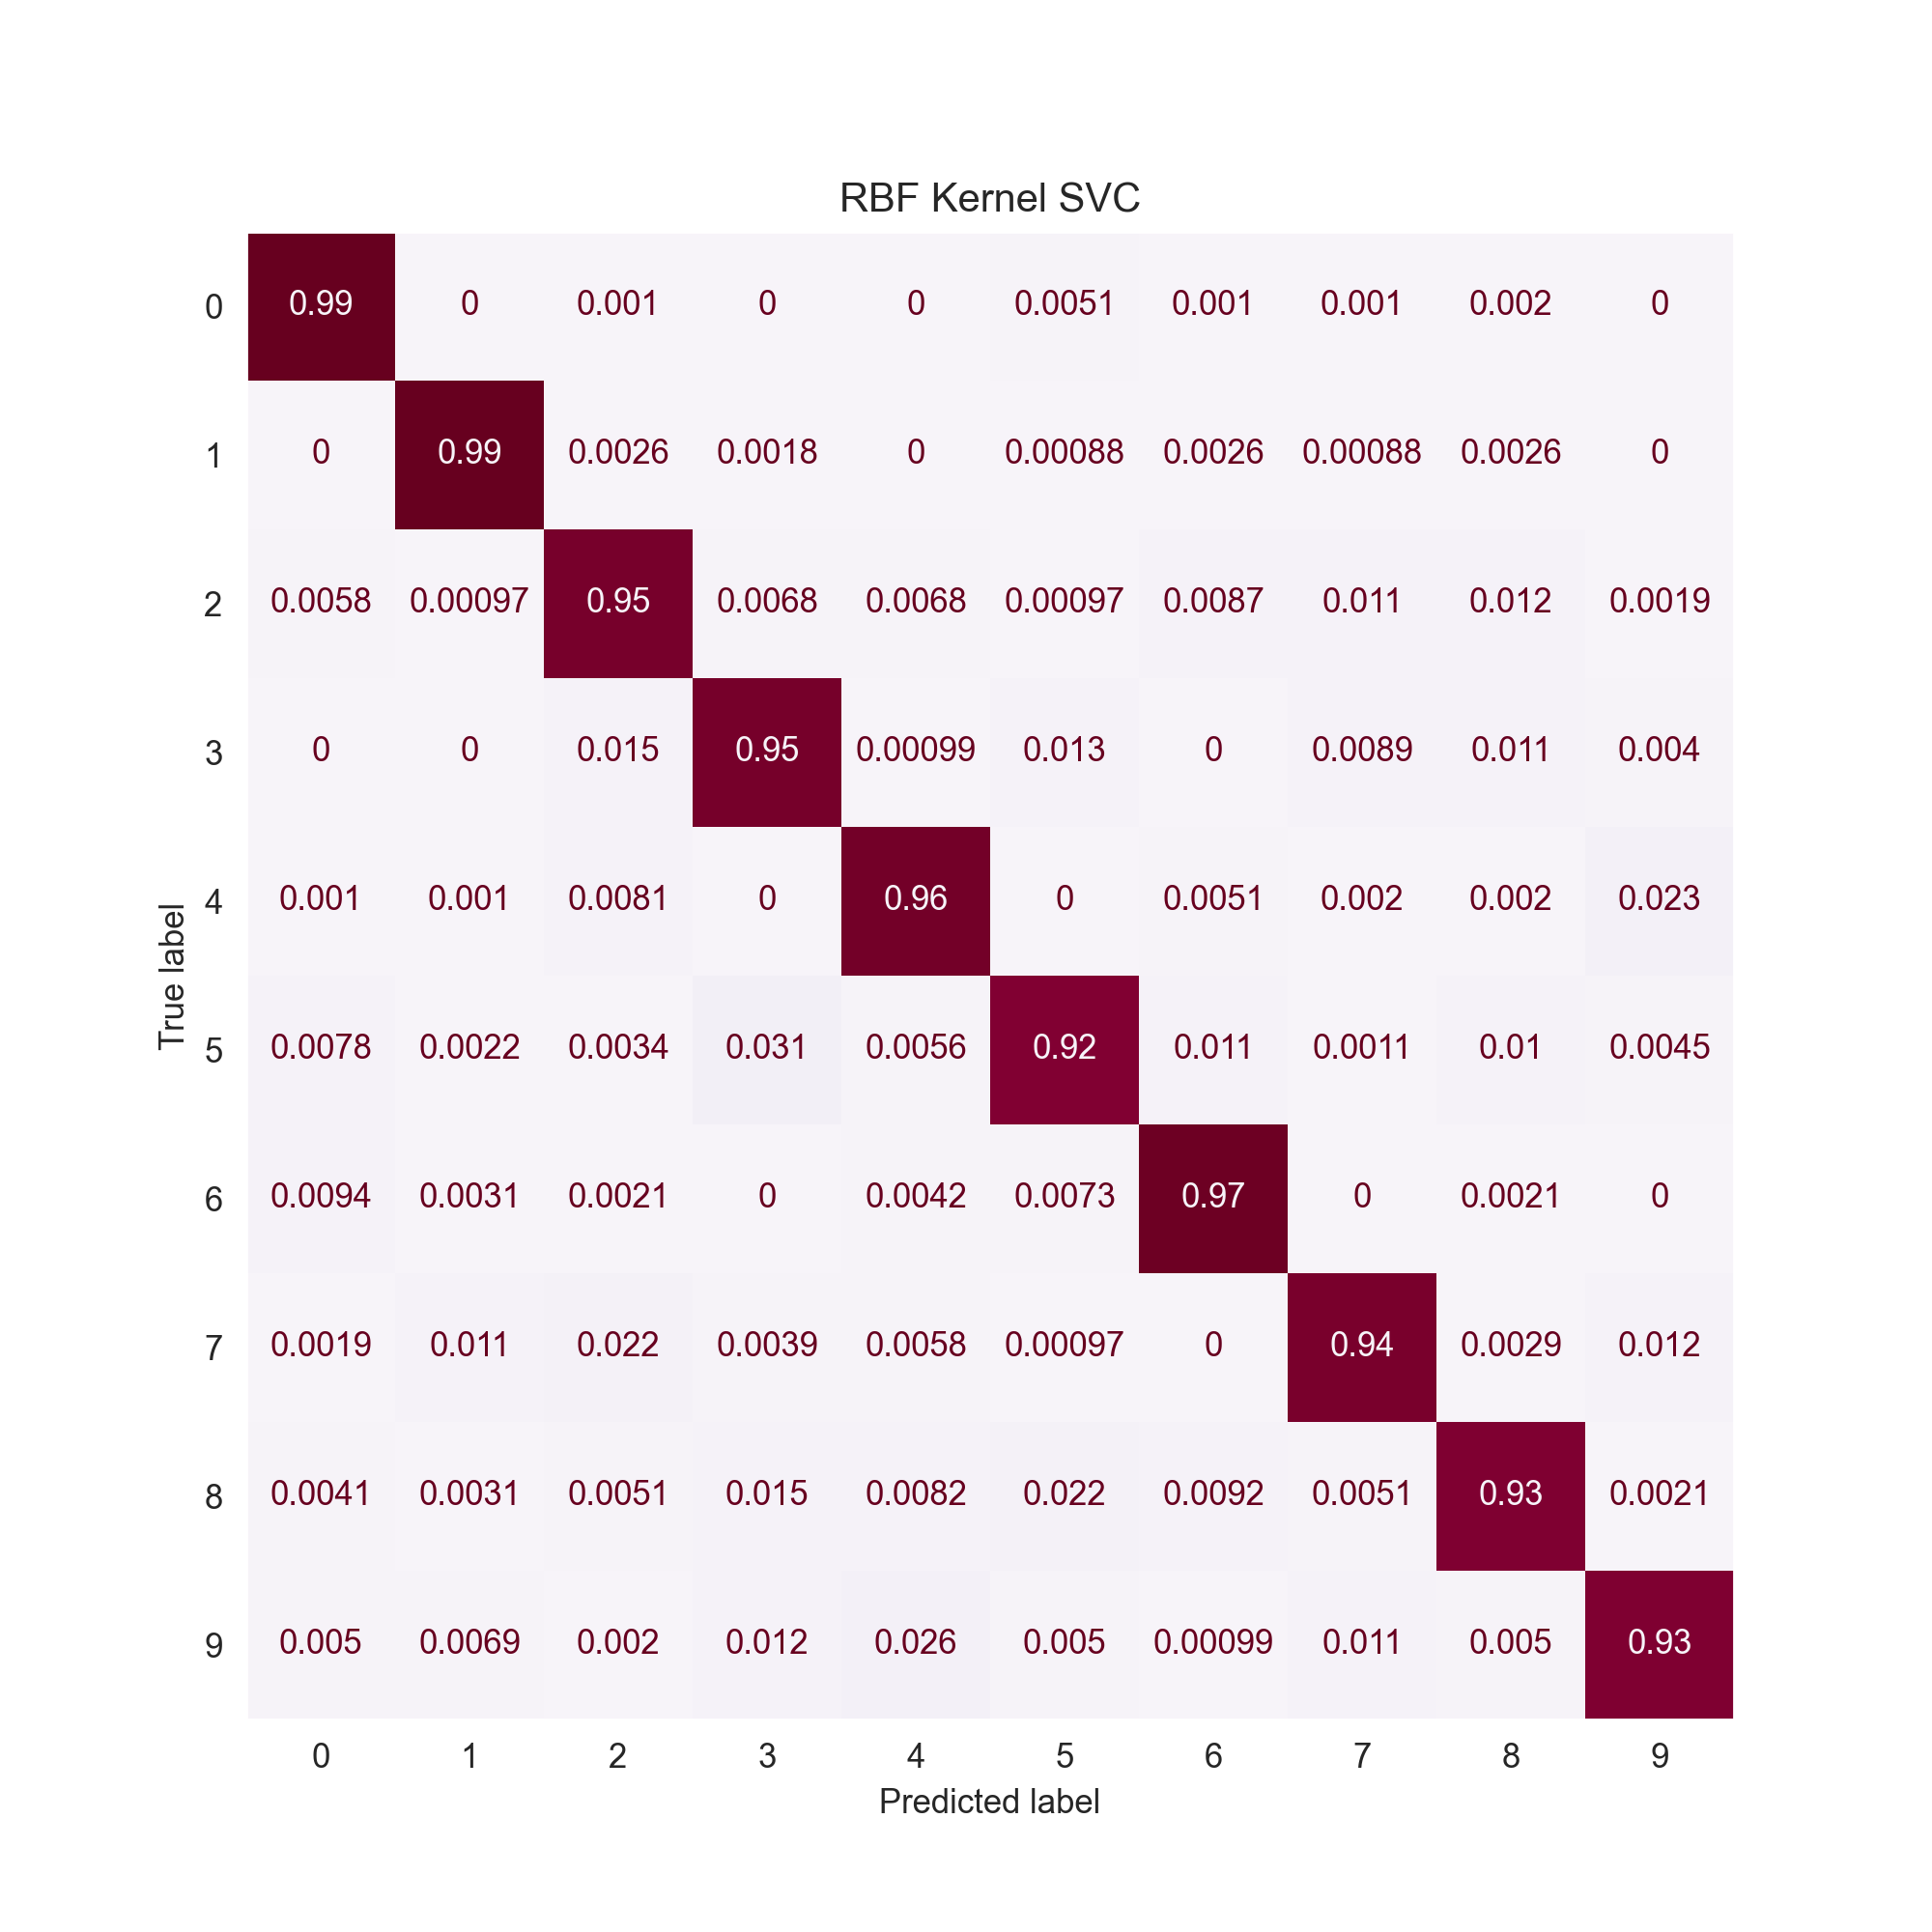
\includegraphics[scale=0.65]{images/exp-results/svm/svc_rbf_conf-matrix.png}
    \caption{Radial Basis Function Kernel SVM confusion matrix}
    \label{fig:exp_res_rbf_svm_conf_mat}
\end{figure}


\newpage
\section{KNN}

\subsection{Implementation}

The \textit{KNN} classifier was \textit{manually} implemented by adhering to \textit{Sci-kit learn}'s \textit{BaseEstimator} API, so that it would be compatible with all the utilities provided by the aforementioned library. 
The implementation is characterized by a lazy fitting, where the training data is just stored for later, and euclidean distance-based predictions. Although \textit{numpy}'s vectorization capabilities were heavily used, making a prediction is still in the $O(n^2)$ time complexity class, meaning that my implementation was still somewhat slow.

Below are some images related to the core parts of the source code.

\begin{figure}[h]
    \centering
    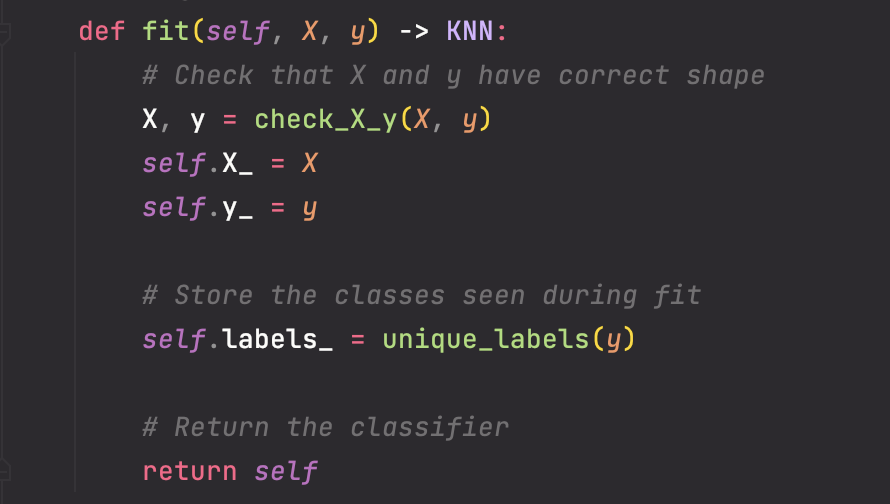
\includegraphics[scale=0.6]{images/exp-results/knn/knn-fit.png}
    \caption{KNN.fit() implementation - source code}
    \label{fig:exp_res_knn_fit}
\end{figure}

\begin{figure}[h]
    \centering
    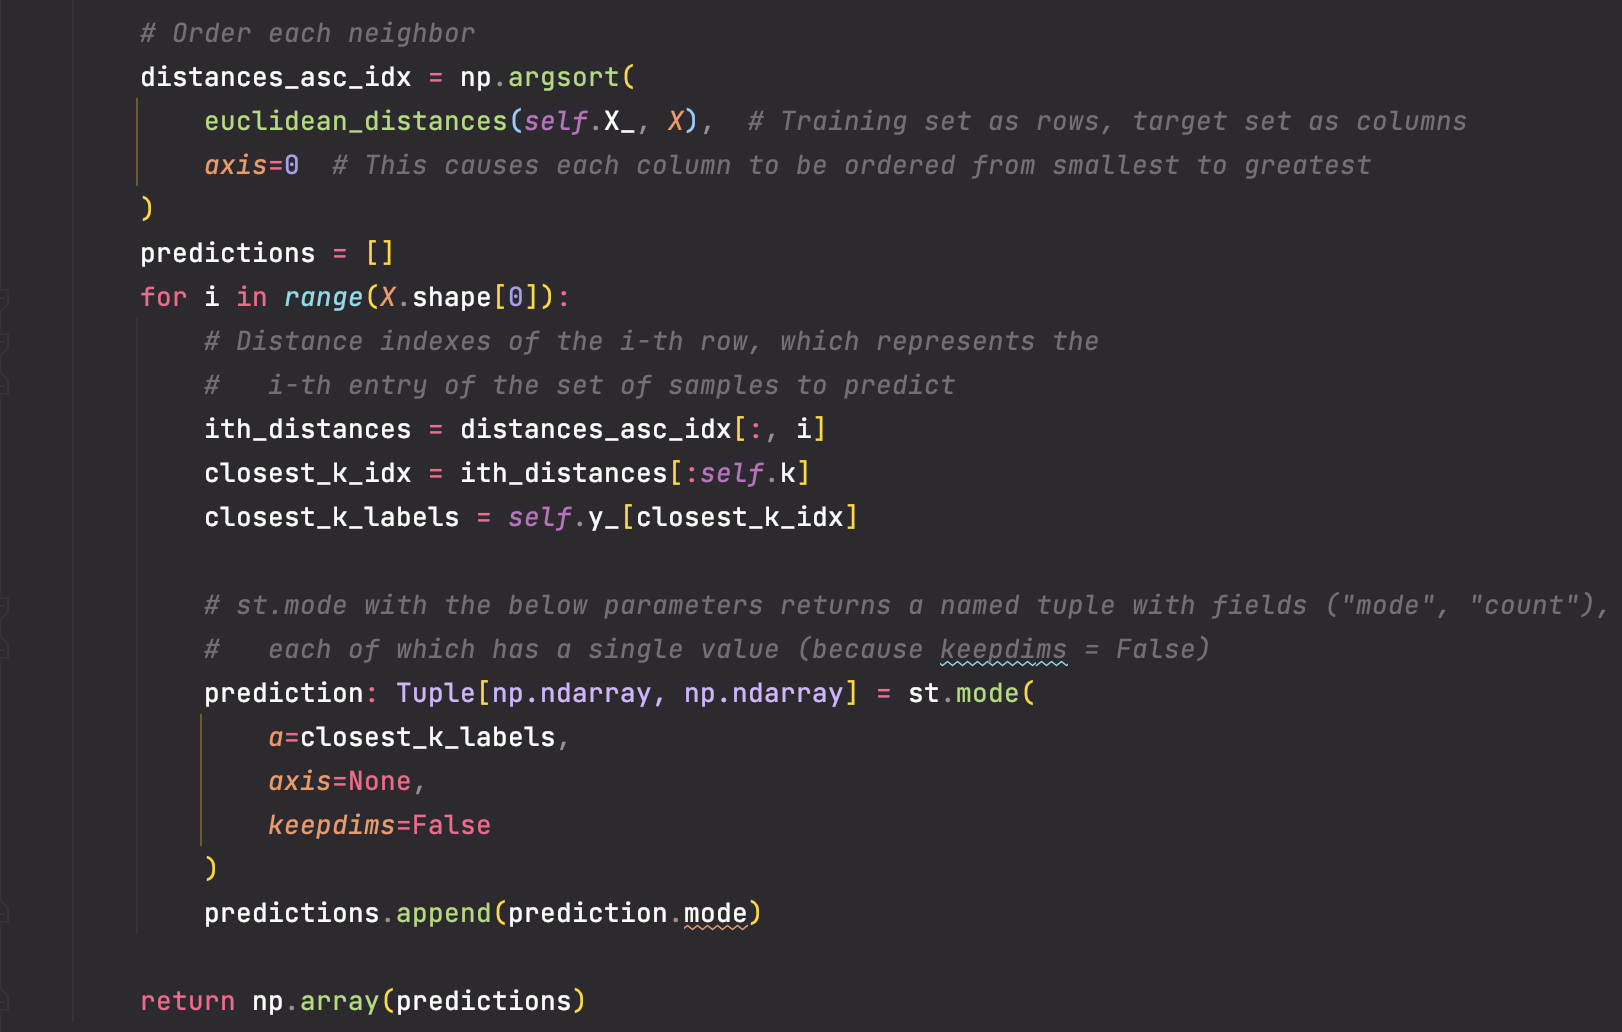
\includegraphics[scale=0.4]{images/exp-results/knn/knn-predict.png}
    \caption{KNN.predict() implementation - source code}
    \label{fig:exp_res_knn_predict}
\end{figure}

\subsection{Hyperparameter Tuning}

This implementation relied on only one hyperparameter, that is, $k$, the number of neighbors. For this reason, it was the only one optimized with the grid search. The set of values that were tried is the following:

\begin{lstlisting}[language=json]
{
    "k": [5, 10, 25, 50, 100, 200]
}
\end{lstlisting}

\paragraph{Best Parameters} The best value of $k$ was found to be $5$

\subsection{Performance Metrics}

\paragraph{Overall Accuracy} The overall accuracy of the model was $98.5\%$

\paragraph{Confusion Matrix} Below is the confusion matrix for this model. It can be noted that it performed exceptionally well, at least when compared to the previously analyzed models, with samples belonging to almost every class. It can be seen that it achieve almost 100\% accuracy at labelling 1s, while the worst performing samples were 8s.

\begin{figure}[h]
    \centering
    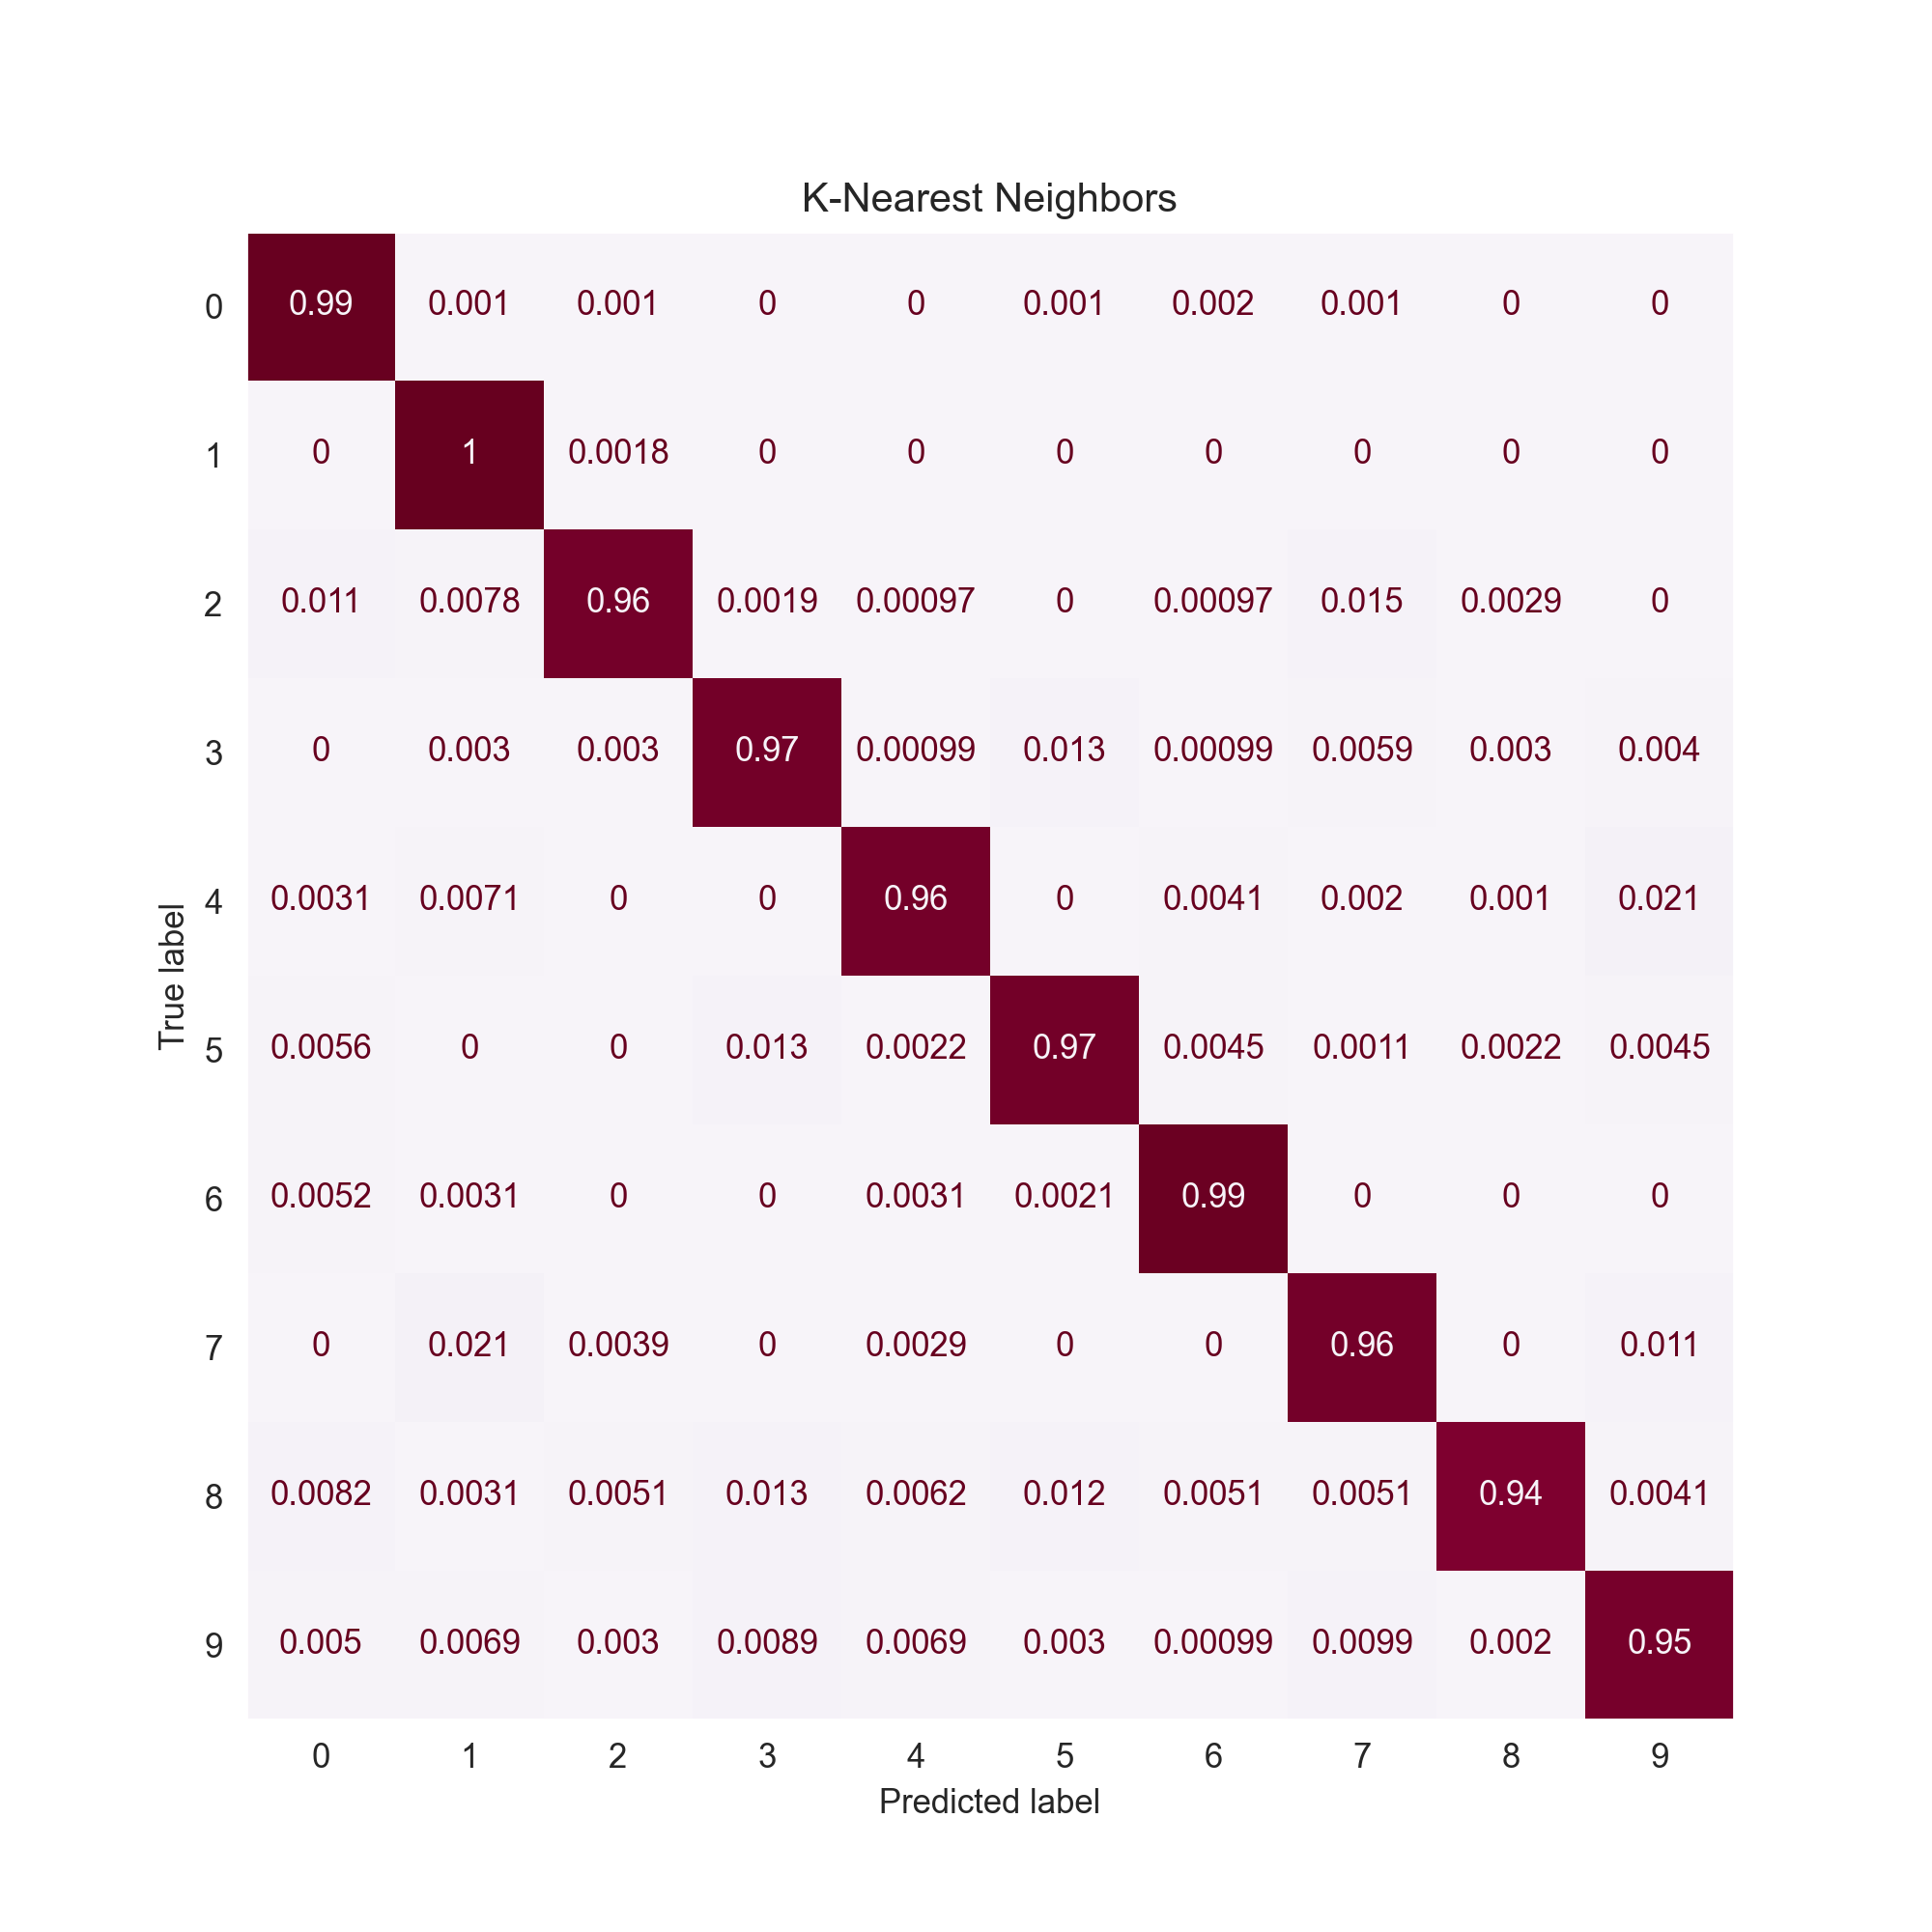
\includegraphics[scale=0.65]{images/exp-results/knn/knn_conf-matrix.png}
    \caption{KNN confusion matrix}
    \label{fig:exp_res_knn_conf_mat}
\end{figure}


\newpage
\section{Beta Distribution Naive Bayes}

\subsection{Implementation}

As was the case with \textit{KNN}, the Beta Distribution Naive Bayes classifier, represented by the \textit{BetaNaiveBayes} class in the source code, was implemented to leverage sklearn utilities, hence it adhered to the \textit{BaseEstimator} API.
The paragraphs below discuss the main parts of the implementation, i.e. the fitting and prediction functionality of the classifier.

\paragraph{Fitting} The \textit{fit(X, y)} method of the classifier, responsibile of building it by using the training samples and labels $X$ and $y$, mainly consisted of estimating the $\alpha$ and $\beta$ parameters of $719 \cdot 10 = 7190$ Beta distributions, that is, one distribution for each pair of feature and label.
The parameters estimation was done by using the moments approach, as suggested in the assignment instructions. It is recalled that the mathematical formulas to estimate each parameter are the following:

$$
\begin{aligned}
    & \alpha = KE[X] \\
    & \beta = K(1 - E[X]) \\
    & K = \frac{
        E[X](1 - E[X])
    }{
        Var[X]
    } - 1 \\
\end{aligned}
$$

It is noted that, sometimes, it wasn't possible to estimate the parameters using this approach: some features were constant in value, meaning that their variance was 0 and $K$, as well as $\alpha$ and $\beta$ couldn't be calculated. Such features were marked in order to be handled as a special case in the prediction phase, which will be discussed in the next paragraph.

\begin{figure}[h]
    \centering
    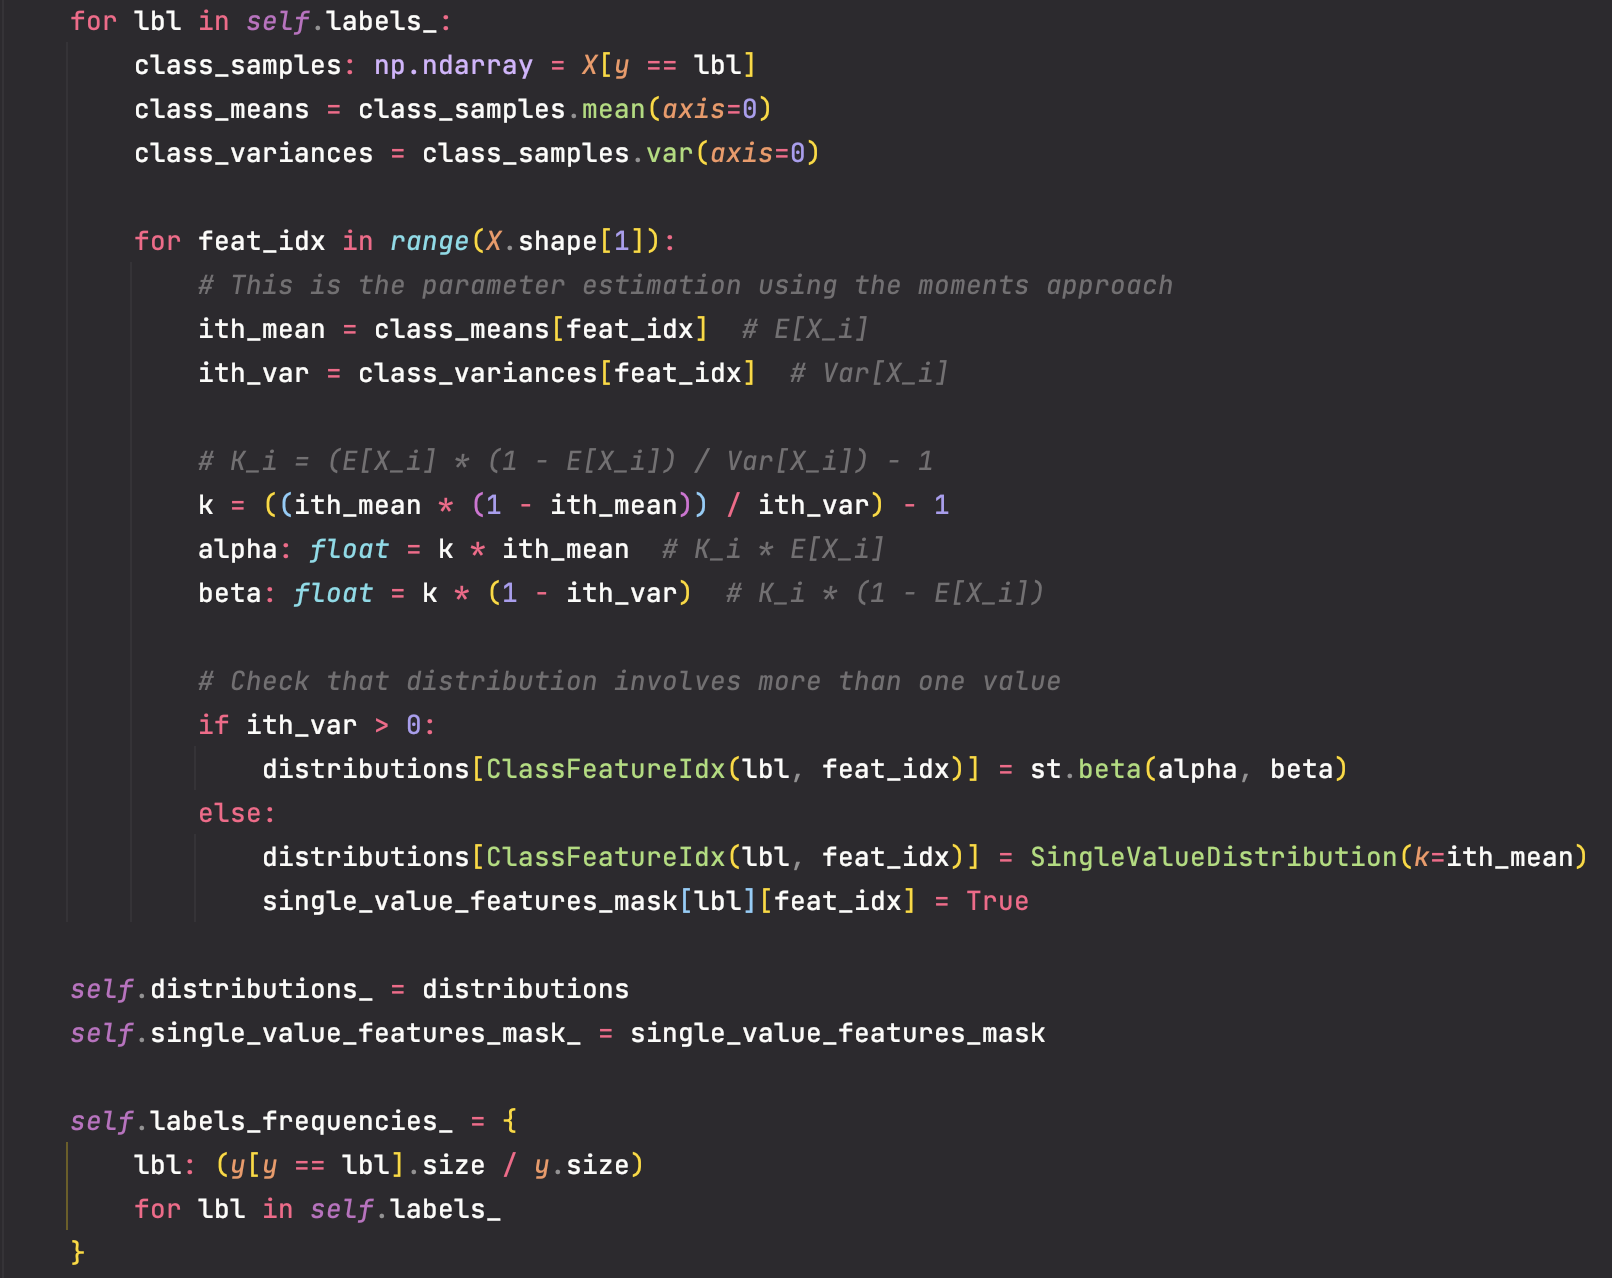
\includegraphics[scale=0.6]{images/exp-results/bayes/bayes-fit.png}
    \caption{BetaNaiveBayes.fit() implementation - source code, core parts}
    \label{fig:exp_res_bayes_fit}
\end{figure}

\paragraph{Predictions} The \textit{predict(X)} method of the classifier, responsible for assigning labels to the samples in $X$, mainly consisted in applying the naive bayes rule, previously explained at \ref{theory_naive_bayes_formula}. When the probability $p(x_i \mid y)$ had to be calculated for features $i$ that, during the training phase, were marked as constant value ones, such a probability was explicitly set to $1$, in order to make it an irrelevant term in the product of the conditional probabilities (refer to \ref{theory_naive_bayes_formula}); this is because a Beta distribution for such features couldn't be properly estimated.

\begin{figure}[h]
    \centering
    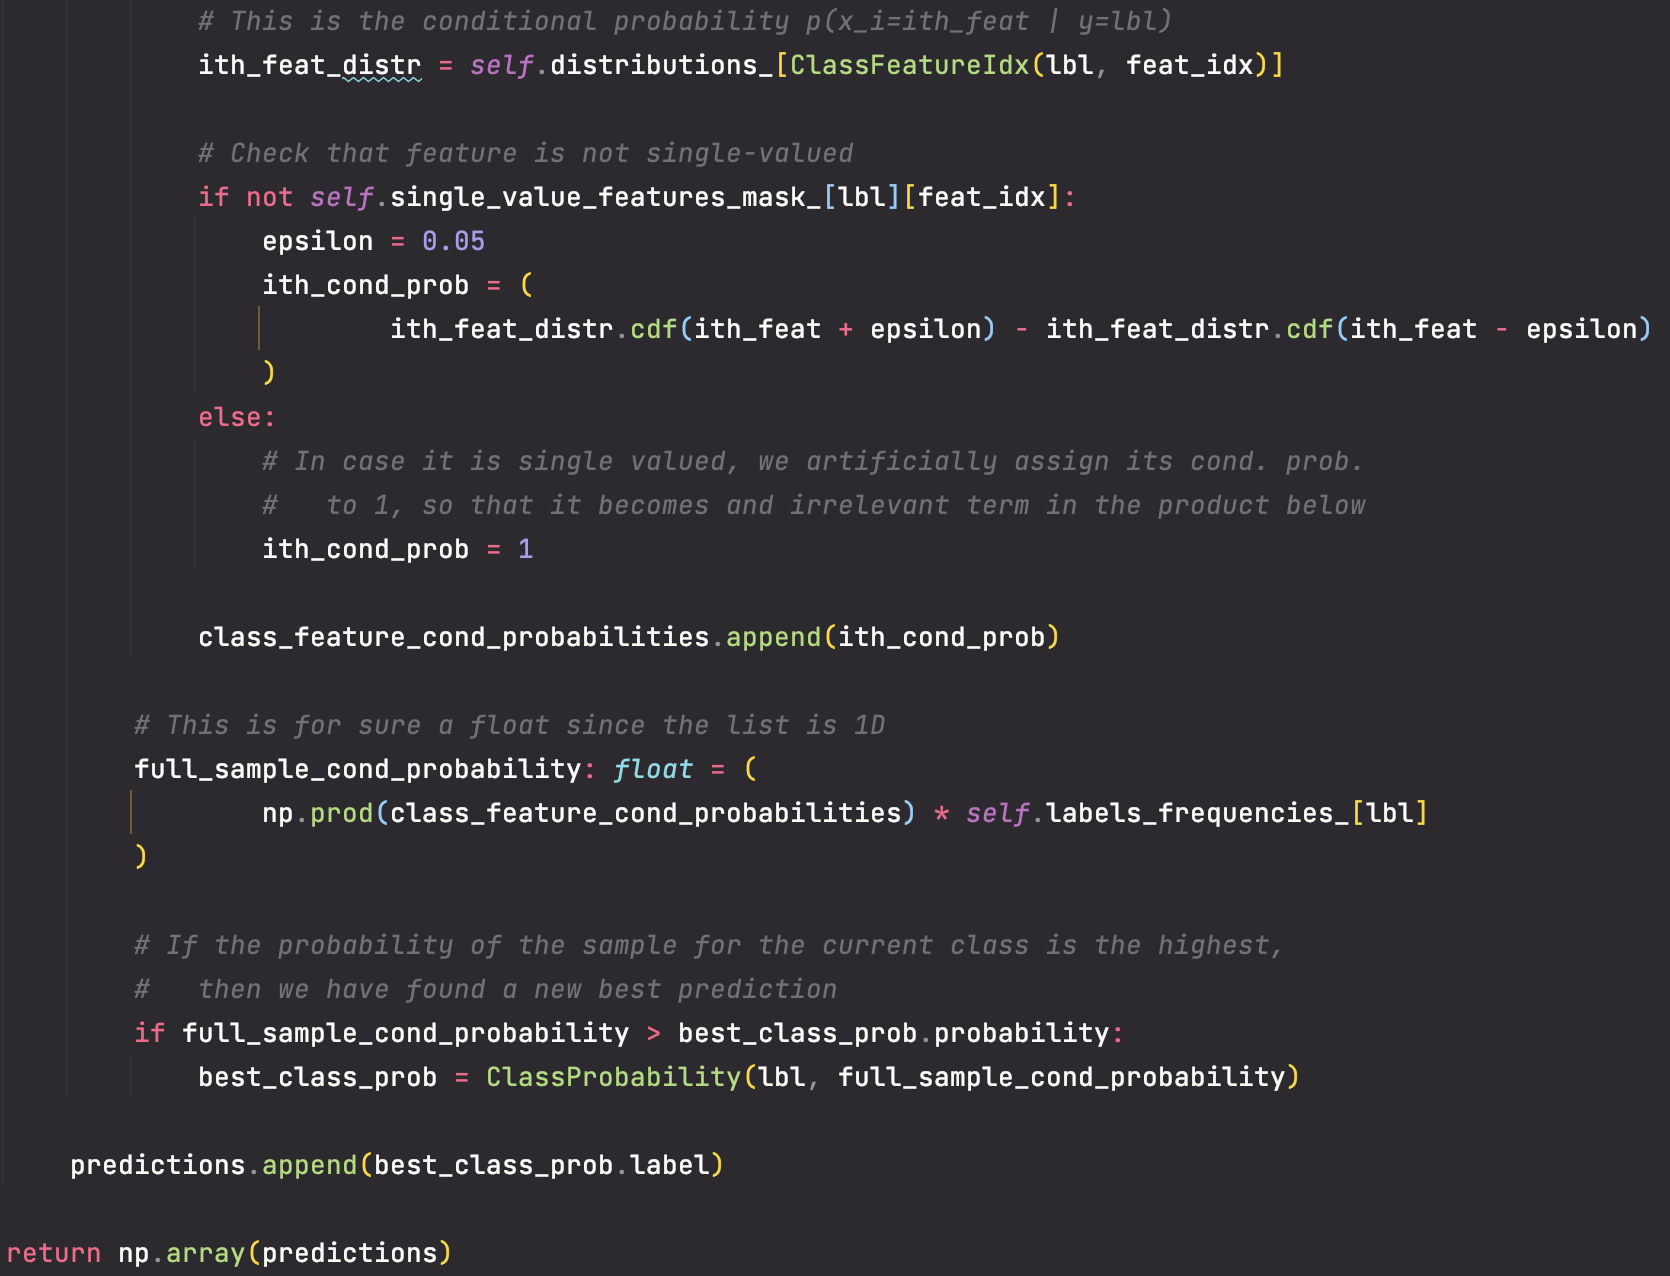
\includegraphics[scale=0.55]{images/exp-results/bayes/bayes-predict.png}
    \caption{BetaNaiveBayes.predict() implementation - source code, core parts}
    \label{fig:exp_res_bayes_predict}
\end{figure}


\subsection{Hyperparameter Tuning}

This implementation had no hyperparameters, so this part was skipped.

\subsection{Performance Metrics}

\paragraph{Overall Accuracy} The overall accuracy of the model was $84.2\%$

\paragraph{Confusion Matrix} Below is the confusion matrix for the \textit{Polynomial Kernel SVM}. It can be noted that it performed quite worse when compared to the previosuly discussed classifiers, being particularly troubled at correctly labelling instances of 4s, 5s and 8s.

\begin{figure}[h]
    \centering
    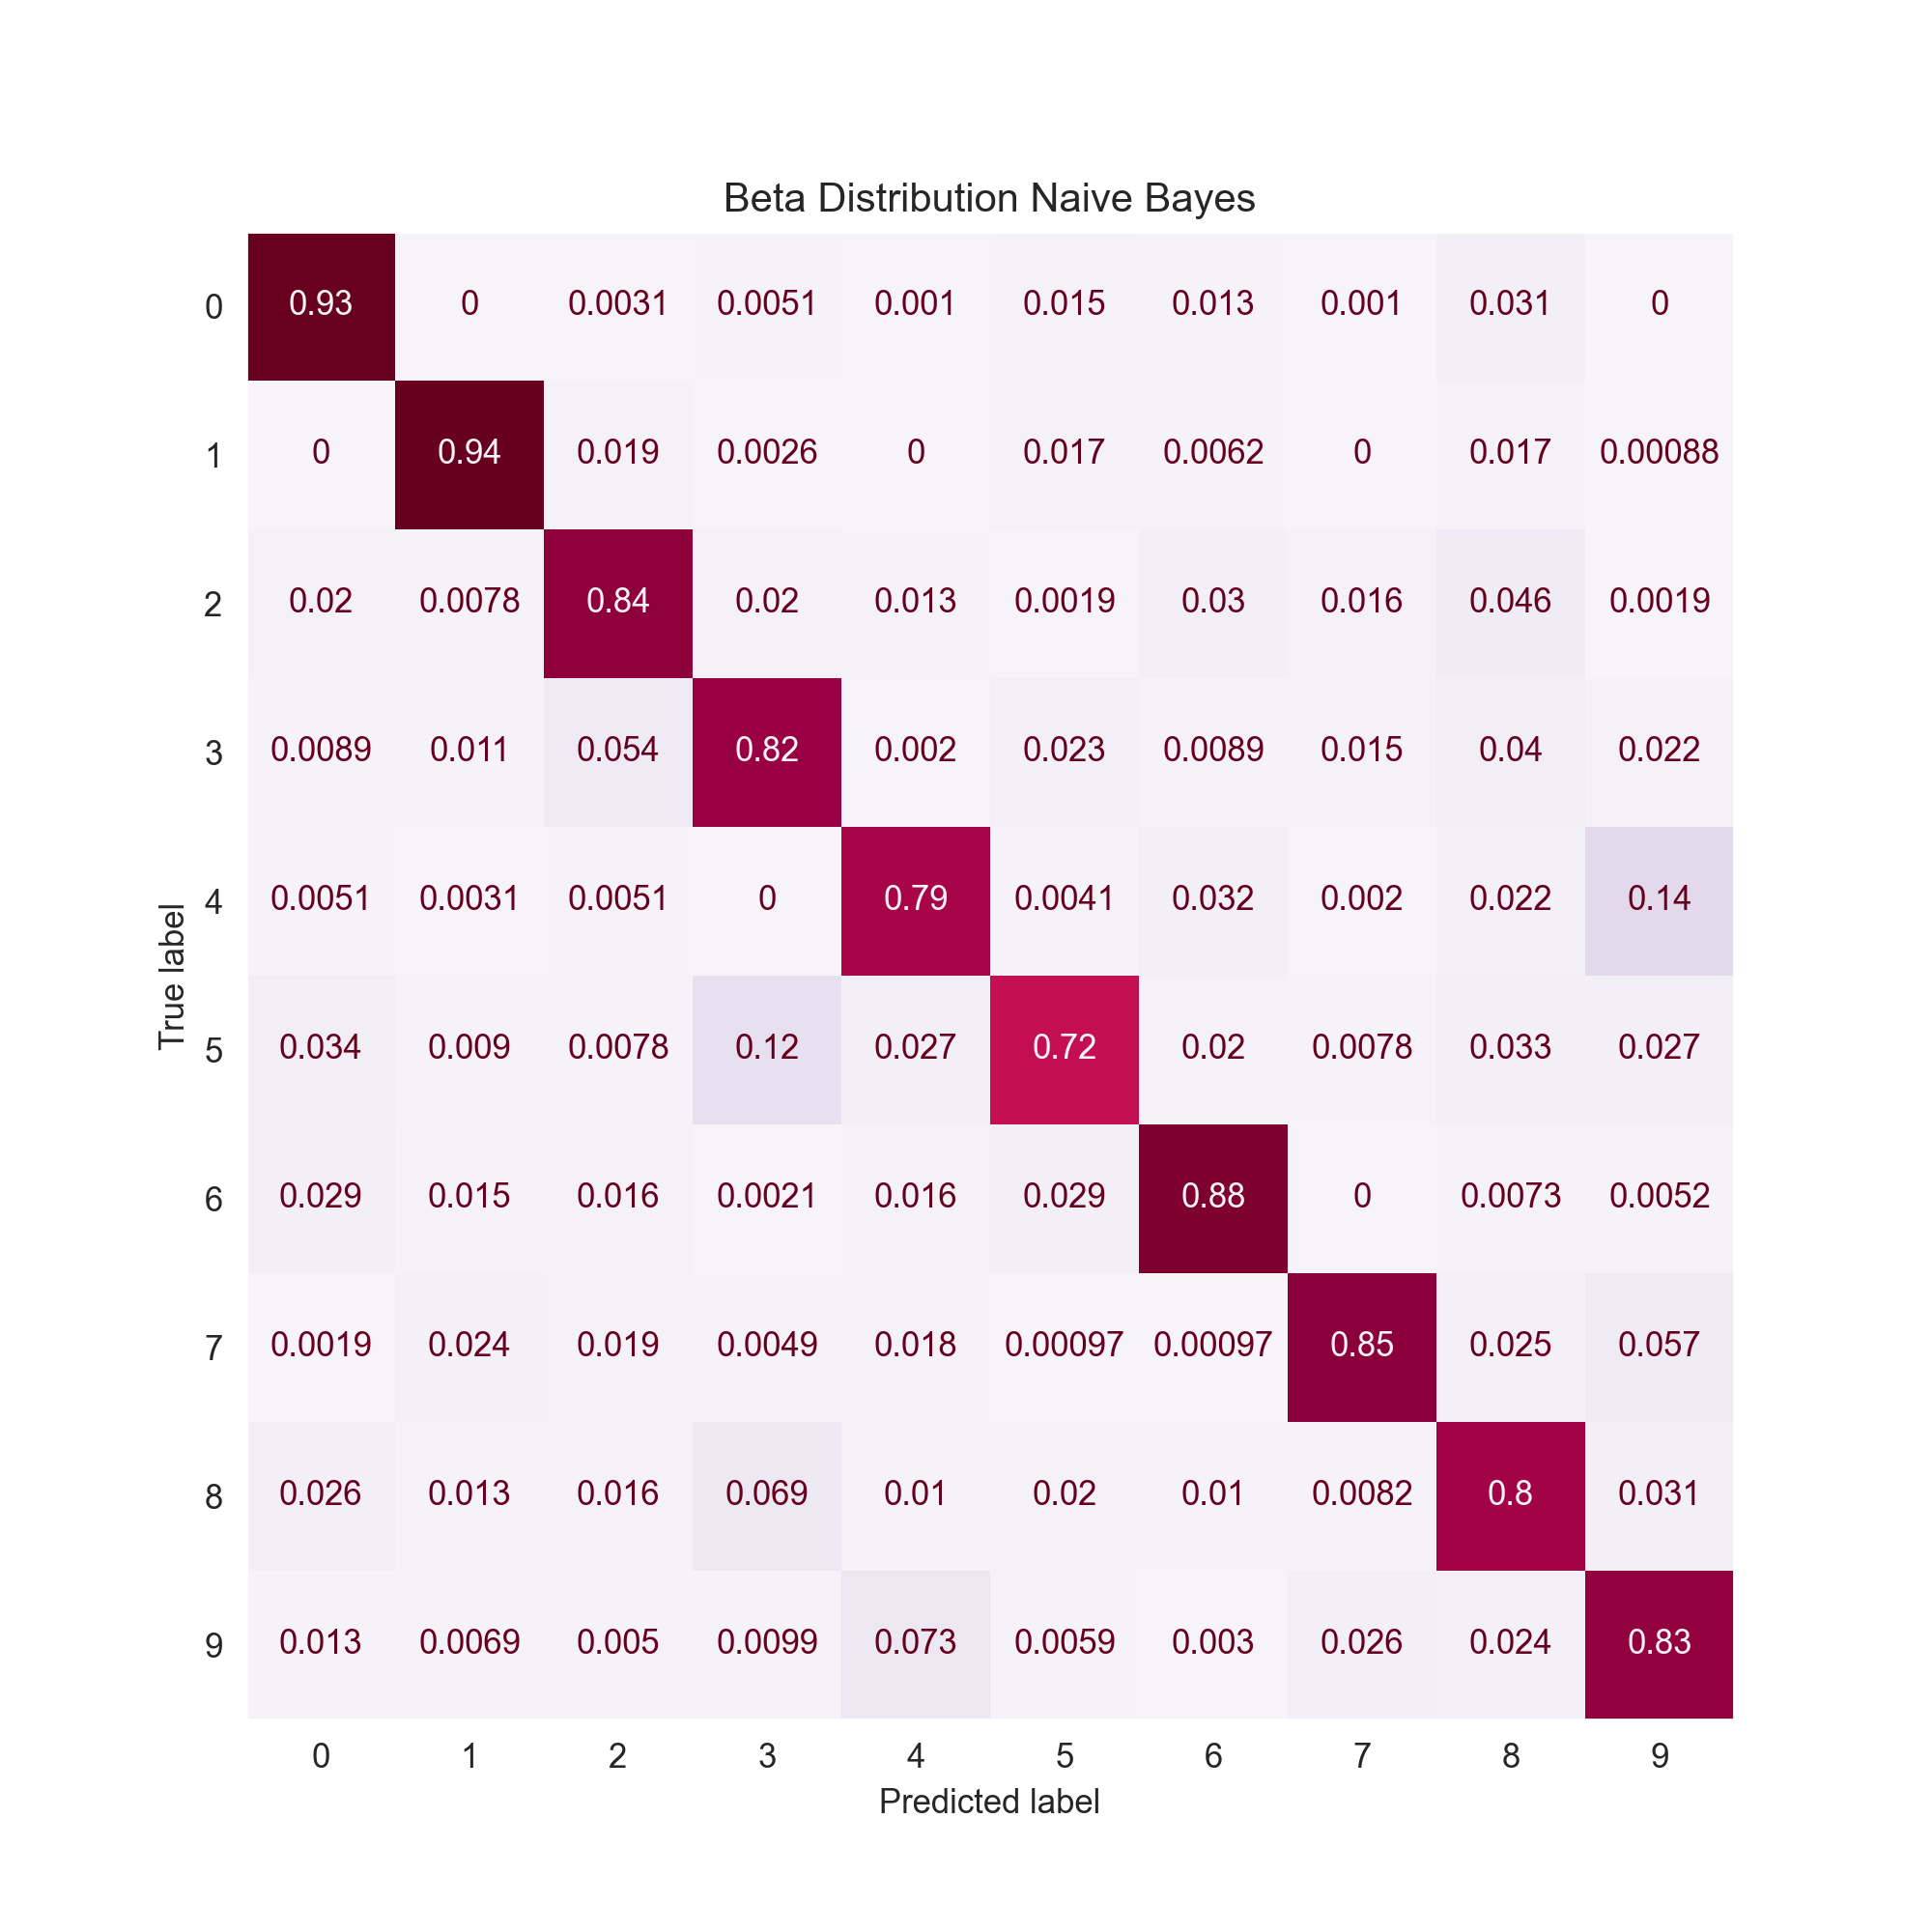
\includegraphics[scale=0.65]{images/exp-results/bayes/beta_bayes_conf-matrix.png}
    \caption{Beta Distribution Naive Bayes confusion matrix}
    \label{fig:exp_res_bayes_conf_mat}
\end{figure}

\subsection{Mean Images}

The following is a set of images, one for each digit, obtained by plotting the mean of each pixel, for each class, of the estimated beta distribution. In a sense, this is what the \textit{BetaNaiveBayes} classifier \textit{"sees"} on average.

\begin{figure}[h]
    \centering
    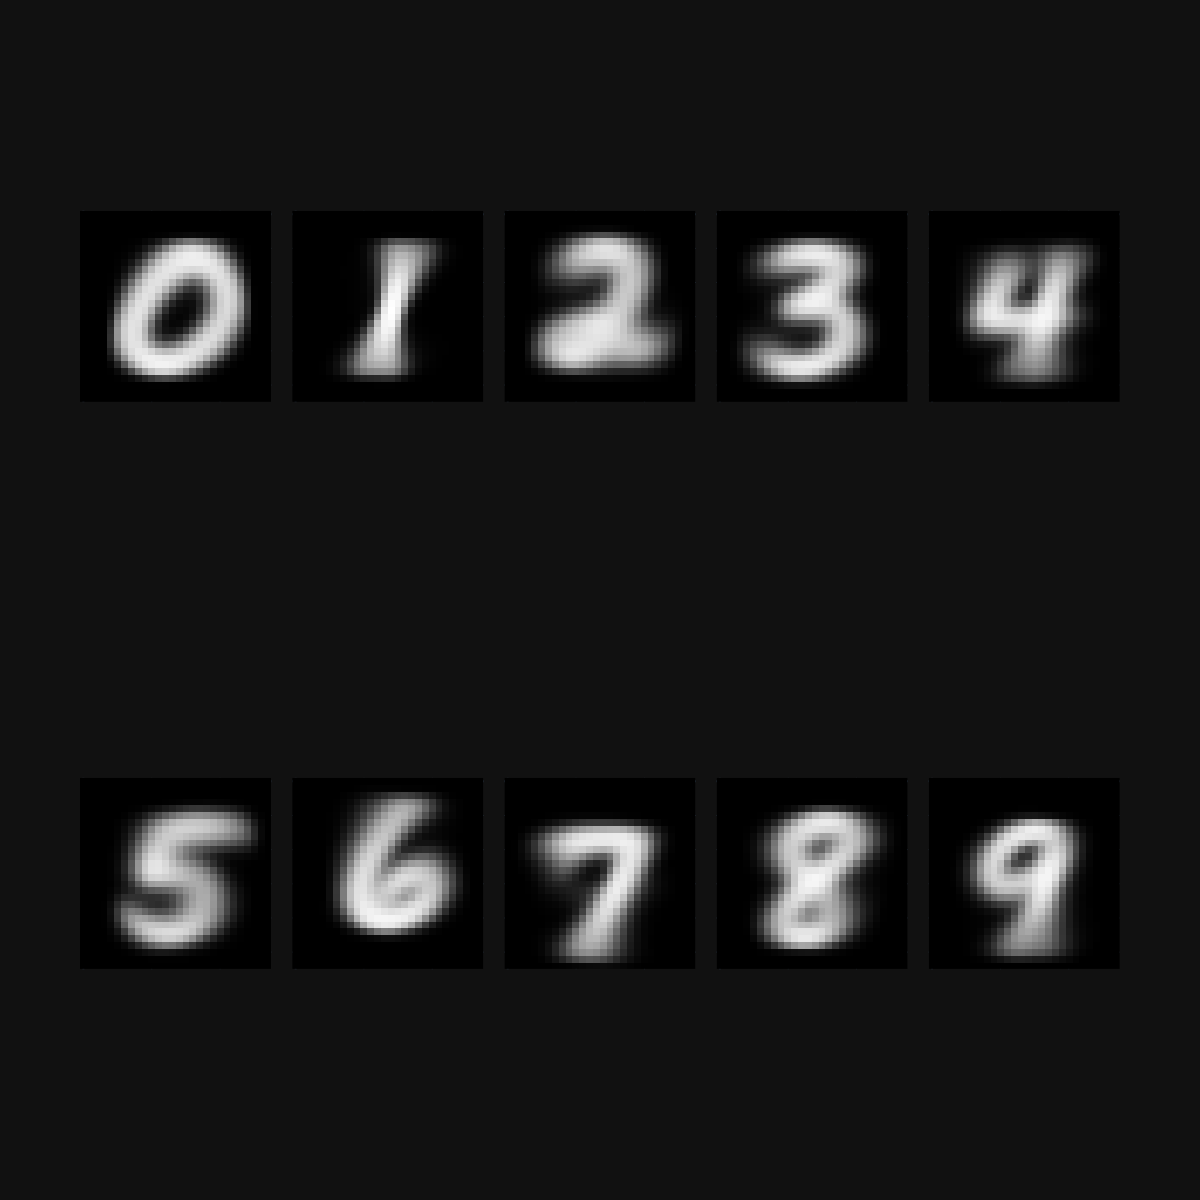
\includegraphics[scale=0.25]{images/exp-results/bayes/beta_means.png}
    \caption{Images that represent the mean of the Beta distributions estimated by the \textit{BetaNaiveBayes} classifier}
    \label{fig:exp_res_bayes_beta_means}
\end{figure}


\newpage
\section{General Considerations on Classification Accuracy}

It seems to be the case that every model performs better when the classification task involves instances of 0s and 1s, while the accuracy drops, even drammatically, if instances of other numbers are to be labelled, especially 5s and 8s. 
This, however, is intuitive, because the distinguishing characteristics of digits from 2 to 9 are similar, and, in some cases, overlapping. Such an overlap is highlighted by misclassification errors, for example, when classifiers label an instance a 3 when it really is a 5. As regards to 0s and 1s, instead, they are quite different from each other and all the other digits, at least in the way they are represented in the dataset used for this assignment.


